% \documentclass[journal = jpccck, manuscript = article]{achemso}
% \setkeys{acs}{usetitle = true}
% \usepackage{fixltx2e}
% \usepackage{float}
% \usepackage{achemso}
% \usepackage{natbib}
% \usepackage{multirow}
% \usepackage{wrapfig}
% \usepackage{times}
% \usepackage{tablefootnote}
% \usepackage{booktabs}
% \usepackage[version=3]{mhchem}  % this is a great package for formatting chemical reactions
% \usepackage{url}
% \usepackage{graphicx}  % needed for figures
% \usepackage{dcolumn}   % needed for some tables
% \usepackage{bm}        % for math
% \usepackage{amssymb}   % for math
% \usepackage{booktabs}
% \usepackage{tablefootnote}
% \usepackage{mathptmx}

\newcommand*{\citen}[1]{%
  \begingroup
    \romannumeral-`\x % remove space at the beginning of \setcitestyle
    \setcitestyle{numbers}%
    \cite{#1}%
  \endgroup   
}

\chapter{FRICTION AT ICE-I$_\mathrm{h}$ / WATER INTERFACES IS GOVERNED
  BY SOLID / LIQUID HYDROGEN-BONDING}

% \title[Friction at Ice-I$_\mathrm{h}$ / Water Interfaces]{Friction at
%   Ice-I$_\mathrm{h}$ / Water Interfaces is Governed by Solid / Liquid
%   Hydrogen-Bonding}
% \author{Patrick B. Louden}
% \author{J. Daniel Gezelter} \email{gezelter@nd.edu} \phone{+1 (574) 631-7595}
% \affiliation{Department of Chemistry and Biochemistry, University of
%   Notre Dame, Notre Dame, IN 46556} 

% \keywords{ice; water; interfaces; friction; hydrogen bonding}

% \begin{document}

% \begin{tocentry}
% \center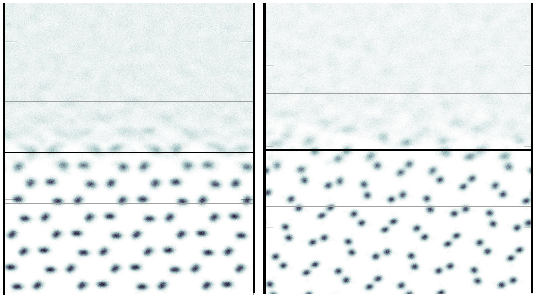
\includegraphics[width=2.55in]{TOC.pdf} 
% \end{tocentry}

% \begin{abstract}
Non-equilibrium molecular dynamics simulations of solid / liquid
friction at ice / water interfaces suggest that the surface density
of solid to liquid hydrogen bonds directly correlates with
interfacial friction.  The basal $\{0001\}$, prismatic
$\{10\bar{1}0\}$, pyramidal $\{20\bar{2}1\}$, and secondary prism
$\{11\bar{2}0\}$ facets of ice-I$_\mathrm{h}$ were drawn through
liquid water with a momentum flux between the solid and liquid
phases. Solid to liquid hydrogen bonds were identified using local
tetrahedral ordering of the water molecules. An expression for
friction coefficients appropriate for negative slip boundary
conditions is presented, and the computed friction of these
interfaces is found to be invariant to the shear rate and direction
of shear relative to the surface features. Structural and dynamic
interfacial widths for all four facets were found to be similar
(6.6--9.5 \AA~structural, 9--15 \AA~dynamic), and are largely
independent of the shear rate and direction. Differences in the
solid to liquid hydrogen bond density are explained in terms of
surface features of the four facets. Lastly, we present a simple
momentum transmission model using the density of solid / liquid
hydrogen bonds, the shear viscosity of the liquid, and the
structural width of the interface.
%\end{abstract}


\section{Introduction}

Ice friction has been investigated extensively with a range
of experimental techniques to elucidate the role of
temperature,\cite{Bowden1939,Evans1976,Roberts1981,Derjaguin1988,Liang2003,Higgins2008} sliding speed,\cite{Evans1976,Derjaguin1988,Liang2003} applied
load,\cite{Bowden1939,Oksanen1982,Derjaguin1988,Buhl2001,Baurle2006}
contact area,\cite{Bowden1939,Baurle2007} and
moisture.\cite{Calabrese1980} Kietzig \textit{et al.} performed
experiments on steel alloy rings sliding over a prepared ice
surface.\cite{Kietzig2009} They investigated the effect of surface
nanopatterning, hydrophobicity, and surface structure of the
ice-exposed slider on the ice / slider friction.
Using laser irradiation, the slider surface hydrophobicity was tuned
without changing the chemical nature of the material. Kietzig showed
that laser-induced hydrophobicity resulted in fewer capillary bridges
forming between the slider and a thin film of melted ice. This reduced
the amount of viscous shearing of the ice-melt, resulting in a lower
friction coefficient.
While ice friction experiments have focused on heterogeneous
materials,\cite{Bowden1939,Evans1976,Derjaguin1988,Liang2003,Liang2005,Baurle2006,Baurle2007,Kietzig2009,Kietzig2010}
there have also been significant advances made in understanding
ice-ice
friction.\cite{Oksanen1982,Kennedy2000,Maeno2004,Fortt2007,Fortt2011,Lishman2011,Samadashvili2013}

Experiments and computer simulations both suggest the existence of a
quasi-liquid layer (QLL) that forms at the surface of ice at
temperatures below the bulk melting point but above
235~K.\cite{Kroes1992,Ikeda-Fukazawa2004,Picaud2006,Conde2008,Bartels-Rausch2014,Sancheza2017}
The formation of this layer is driven by the termination of the
periodic crystal structure. The surface molecules are not as tightly
bound to their lattice positions as molecules in the underlying ice,
and with sufficient thermal energy, these molecules reorient to
maximize hydrogen bonding. At warmer temperatures, they can also
translate along the surface.\cite{Pfalzgraff2011,Bartels-Rausch2014}
The existence of the QLL is now generally accepted as one of the
reasons that ice displays a low coefficient of sliding
friction.\cite{Dash1995,Rosenberg2005,Dash2006,Malenkov2009}

Three distinct ice friction regimes have been described:
boundary friction, mixed friction, and hydrodynamic friction, and the
particular regime depends on the temperature and sliding velocity of
the
material.\cite{Bhushan2002,Kietzig2009,Kietzig2010,Persson2015,Tuononen2016}
The observed friction is the result of different physical processes in
each regime. In boundary friction, the lubricating layer of ice melt
is only a few molecules thick. This thin film is unable to support the
sliding load, and friction can be attributed to surface asperities of
the sliding material interacting with the ice surface
itself.\cite{Bhushan2002} In the mixed friction regime, the
lubricating layer is thicker than in the boundary regime, but not yet
sufficiently thick to maintain the sliding load. The QLL film reduces
solid-solid adhesion at the interface, although the lubricating layer
can also form capillary bridges with the material, resulting in a drag
force.\cite{Kietzig2009,Kietzig2010}

If the liquid layer is thick enough to support the sliding load, the
slider's surface asperities are no longer in contact with the surface
and the observed friction may be partially due to the capillary
bridges formed between the ice melt and the material. Under these
conditions, the ice friction is classified as hydrodynamic
friction.\cite{Kietzig2009,Kietzig2010} Thus the three regimes are
characterized by the extent that a liquid-like layer of water
mitigates the sliding load.

\begin{figure}
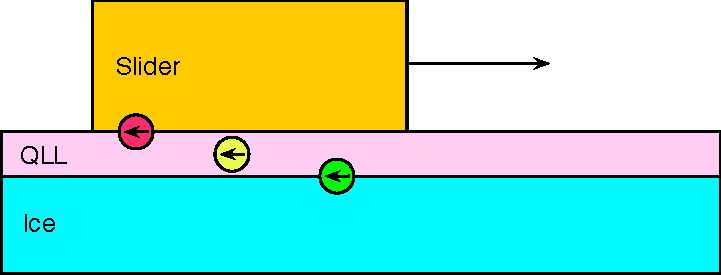
\includegraphics[width=4in]{Figures/QLLsketch}
\caption{\label{fig:QLLsketch} In the hydrodynamic regime, the
  friction felt by a slider on an ice surface is mediated by a
  quasi-liquid layer (QLL) that forms on the surface of the ice.
  There can be many contributions to this friction: capillary bridges
  between the slider and the QLL (red), viscous drag in the liquid
  (yellow), and solid / liquid friction between the ice and the liquid
  film (green). This study concerns the last of the three
  contributions, the drag contributed by the ice-liquid interface.}
\end{figure}

Kietzig \textit{et al.} have outlined popular experimental techniques
used to investigate the coefficients of friction for a variety of
materials sliding on ice, as well as their sensitivity to temperature,
slider load, contact area, wettability and hydrophobicity of the
slider.\cite{Kietzig2010} Of particular interest, the friction
coefficients were found to increase with increasing slider
velocity. This was attributed to three physical processes; adhesion
forces between the slider's asperities and the ice surface, breaking
of capillary bridges between the slider and the ice surface, and the
viscous shearing of the ice melt across the ice surface. While teasing
apart the individual contributions has proven challenging,
Kietzig\cite{Kietzig2009} and Persson\cite{Persson2015,Tuononen2016}
have made significant progress. However, there is still very little
known about water shearing over ice surfaces. Open questions include:
how does the structure of the interface change during this process,
and what role does the presented crystal facet have in the observed
friction?

To help understand slider-ice friction in the hydrodynamic regime, we
have simulated the drag forces contributed by the interaction of the
liquid water film with the underlying ice facet. This study uses
non-equilibrium molecular dynamics (with an applied momentum flux) to
create a shear flow at the ice / water interface. The magnitude of the
momentum flux is then used to compute the solid / liquid friction for
four different facets of ice that are presented to the liquid.  We
have previously used this technique to study solid / liquid friction
for the basal and prismatic crystal facets where we observed
significant facet-dependence, and noted surface corrugations that
could contribute to these differences.\cite{Louden2013a} Here, we
broaden the investigation to four common ice facets using two
different water models, we study significantly larger systems for
significantly longer times, a wider range of shear rates, and we
introduce a novel method for calculating solid / liquid friction
coefficients under conditions of \textit{negative} slip.

\section{Methodology}
\subsection{Construction of Ice / Water interfaces}
%%% Old here
Ice-I$_\mathrm{h}$ crystallizes in the hexagonal space group
P$6_3/mmc$, and ice crystals normally form hexagonal plates with the
basal face, $\{0001\}$, forming the top and bottom of each plate, and
the prismatic facet, $\{10\bar{1}0\}$, forming the sides.  In extreme
temperatures or low water saturation conditions, ice crystals can form
hollow columns, needles, and dendrites, exposing other crystalline
facets of the ice to the surroundings.  Among the more
commonly-observed facets are the secondary prism, $\{11\bar{2}0\}$,
and pyramidal, $\{20\bar{2}1\}$, faces.

The oxygen lattice is a hexagonal unit cell comprising 4 oxygen atoms,
but it is also possible to construct an equivalent orthorhombic unit
cell with 8 oxygen atoms.\cite{Hirsch2004} Hydrogen atom placement
obeys the Bernal-Fowler ice rules which distribute protons so that
each oxygen donates two hydrogen bonds and accepts two from
neighboring molecules.\cite{Bernal1933} The resulting structure also
typically has zero net dipole moment. Below 72~K and under ambient
pressures, the lattice can undergo a phase transition to ice XI, a
configuration with ferroelectric proton-ordering and a non-zero bulk
dipole moment.

While exploring the ice-I$_\mathrm{h}$ to XI phase transition, Hirsch
and Ojam\"{a}e determined sixteen unique hydrogen arrangements for the
ice-I$_\mathrm{h}$ orthorhombic unit cells which yield structures with
zero net dipole.\cite{Hirsch2004} Upon replication of some of these
unit cells, the resulting structures present stripes of dangling
H-atoms and lone pairs at an exposed crystal facet. These orthorhombic
initial configurations can be used to reproduce the surface features
from Buch \textit{et al.}\cite{Buch2008} that helped interpret
sum-frequency generation (SFG) experiments by the Shultz
lab.\cite{Groenzin07} More recently, Nojima \textit{et
  al.}\cite{Nojima2017} have successfully obtained both the real and
imaginary parts of the vibrational spectra of the free OH stretch for
surface water molecules of the basal, prismatic, and secondary
prismatic facets at ca. 130~K through heterodyne-detected
sum-frequency generation (HD-SFG). They also present evidence of
proton-striped surfaces as the sign of the imaginary part of the
vibrational spectra indicates ``up'' or ``down'' orientations of
surface molecules.

SPC/E~\cite{Berendsen1987} and TIP4P/Ice~\cite{Abascal2005} structures
were created starting from Structure 6 of Hirsch and Ojam\"{a}e's set
of orthorhombic representations for ice-I$_{h}$.\cite{Hirsch2004} The
primitive unit cell was replicated in all dimensions. The crystal was
cleaved along the desired face, and two additional mutually
perpendicular cuts were made.  The crystal was reoriented so that the
initial cut (basal, pyramidal, prismatic, or secondary prism) was
normal to the $z$-axis of the simulation cell.  The resulting
structures were extended in $x$ and $y$ to form large exposed facets
in rectangular box geometries.  Because the orthorhombic unit cells
are relatively small, using these as building blocks for an ice
simulation creates proton translational order on the length scale of
the unit cells. We note that all simulated ice structures have proton
ordering on the length scale of the periodic box, but in order to
reproduce proton surface striping with zero dipole crystals, we have
utilized proton translational ordering on a smaller length scale than
other ice studies.

Liquid water boxes were created with identical dimensions (in $x$ and
$y$) as the ice, with a $z$ dimension of three times that of the ice
block, and with a density corresponding to $1$ g / cm$^3$.  Each of
the ice slabs and water boxes were independently equilibrated to
$50$~K and a pressure of $1$ atm by coupling the temperature and
pressure of the system to a heat and pressure bath. For all
simulations non-bonded interactions were cut-off at 12~\AA~ and
electrostatics were handled using the damped-shifted force real-space
electrostatic kernel.\cite{Fennell2006} The resulting systems were
merged by carving out any liquid water molecules within 3~\AA~ of any
atoms in the ice slabs.  For the SPC/E simulations, the combined ice /
water systems were equilibrated to 225~K. The liquid-ice coexistence
temperature for SPC/E water has been reported as
$215 \pm 4$~K.\cite{Vega2006a,Fernandez2006} We observed a coexistence
temperature of 225~K for our crystals, possibly due to the surface
striped structures utilized in this study. For the TIP4P/Ice
simulations, the combined ice / water system was equilibrated to the
reported coexistence temperature, 270~K.\cite{Vega2006a,Fernandez2006}
The quiescent ice / water interfaces were then equilibrated for 10 ns,
with 5 ns under a constant temperature (NVT) integrator, followed by 5
ns under a microcanonical (NVE) integrator.  During this time the ice
was monitored for crystal growth or melting. We observed no advance of
the ice interface into the liquid, and no loss of crystallinity of the
ice. Reference \citen{Louden2013a} contains a more detailed
explanation of the construction of similar ice / water interfaces. The
resulting dimensions as well as the number of ice and liquid water
molecules contained in each of these systems are shown in Table
\ref{tab:sizes}.  Note that the water molecules are not restrained in
any way - molecules that start in the liquid phase may exchange with
the ice (and vice versa).

\begin{table}[h]
\centering
\caption{Sizes of the ice / water shearing simulations. (Box
  dimensions are given in \AA)\label{tab:sizes}}
\begin{tabular}{r|cc|ccc|ccc}
\toprule
 & & & \multicolumn{3}{c|}{SPC/E~(225~K)} &  \multicolumn{3}{c}{TIP4P/Ice~(270~K)}\\
 Interface & $N_\mathrm{ice}$ &
 $N_\mathrm{liquid}$ & $L_x$ & $L_y$ & $L_z$ & $L_x$ & $L_y$ & $L_z$ \\
\midrule
Basal  $\{0001\}$                 & 900 & 1846  & 23.87 & 35.83 & 98.64  & 23.37 & 38.83 & 97.67  \\
Prismatic  $\{10\bar{1}0\}$       & 3000 & 5464 & 35.95 & 35.65 & 205.77 & 36.33 & 38.86 & 191.75 \\
Pyramidal  $\{20\bar{2}1\}$       & 1216 & 2203 & 37.47 & 29.50 & 93.02  & 37.16 & 30.19 & 97.65  \\
Secondary Prism  $\{11\bar{2}0\}$ & 3840 & 8176 & 71.87 & 31.66 & 161.55 & 72.90 & 32.06 & 165.17 \\
\bottomrule
\end{tabular}
\end{table}

The liquid-state viscosity of the SPC/E water model has been
extensively characterized over a wide range of liquid
conditions~\cite{Kuang2012}, and its phase diagram has been well
studied~\cite{Baez1995,Bryk2004,Sanz2004a,Fennell2005}. With longer
cutoff radii and careful treatment of electrostatics, SPC/E mostly
avoids metastable crystalline morphologies like
ice-\textit{i}~\cite{Fennell2005} and ice-B~\cite{Baez1995}, although
Sanz \textit{et al.}\cite{Sanz2004a} found that the stable polymorph
for this model is likely ice-II at this temperature and 1 bar. The
free energies and melting
points~\cite{Baez1995,Arbuckle2002,Gay2002,Bryk2002,Bryk2004,Sanz2004a,Fennell2005,Fernandez2006,Abascal2007,Vrbka2007}
of various other crystalline polymorphs have also been calculated.
Haymet \textit{et al.}\cite{Bryk2002} have studied quiescent
ice-I$_\mathrm{h}$ / water interfaces using the SPC/E water model, and
have seen structural and dynamic measurements of the interfacial width
that agree well with both experimental results and more expensive
water models, although the coexistence temperature for SPC/E is still
well below the experimental melting point of real water.  

Recent investigations have questioned the applicability of SPC/E in
ice / water simulations,\cite{Vega2005c,Vega2011a,Gladich2012,Gallo2016}
however, so simulations have also been done using
TIP4P/Ice.\cite{Abascal2005} This model was parameterized by fitting
the equation of state, as well as the melting and coexistence lines
involving different ice polymorphs, and the resulting melting
temperature of ice-I$_\mathrm{h}$ is much closer to the experimental
value.\cite{Abascal2005} Although TIP4P/Ice is more computationally
demanding, it is worthwhile to compare models where liquid water is in
contact with ice at multiple coexistence temperatures.

\subsection{Creating shear in molecular simulations}
The velocity shearing and scaling variant of reverse non-equilibrium
molecular dynamics (VSS-RNEMD)\cite{Kuang2012} was employed to create
shear in our simulation cells. This method performs a series of
simultaneous non-equilibrium exchanges of linear momentum and kinetic
energy between two physically separated regions of the simulation
cell. The system responds to this unphysical flux with velocity and
temperature gradients. When VSS-RNEMD is applied to bulk liquids,
transport properties like the shear viscosity, $\eta$, are easily
extracted assuming a linear response between the applied flux,
$j_z(p_x)$, and the resulting velocity gradient that develops in the
liquid,\cite{Bordat2002a}
\begin{equation}
\label{eq:viscosity}
j_z(p_x) = -\eta \left(\frac{\partial v_x}{\partial z}\right).
\end{equation}

At interfaces between dissimilar materials, the same method can be
used to extract \textit{interfacial} transport properties (e.g. the
hydrodynamic slip length or the interfacial thermal
conductance). Because the individual VSS-RNEMD exchange moves conserve
both total energy and linear momentum, the method can be ``bolted on''
to simulations in any ensemble.  A more detailed explanation of
VSS-RNEMD shearing simulations applied to ice / water interfaces can
be found in our previous work.\cite{Louden2013a}

All simulations were performed using
OpenMD~\cite{Meineke2005,Gezelter2016}, with a time step of 2 fs and
periodic boundary conditions in all three dimensions. When applicable,
VSS-RNEMD moves were attempted every time step. This minimized the
magnitude of individual momentum exchanges. 

\subsubsection{Shearing at ice / water interfaces}
The RNEMD exchanges that force the solid to shear through a
surrounding liquid do work on the system, and this work causes
frictional heating at the interface. Close to the melting point of the
solid, this frictional heating may result in melting of the crystal.
We are interested in the structure and dynamics of the interface at
the coexistence temperature.  Therefore, in order to prevent melting
of the ice phase, we have imposed a weak kinetic energy flux
($J_z \sim 2.0\times 10^{-6}$~kcal~mol$^{-1}$~\AA$^{-2}$~fs$^{-1}$)
normal to the interface. The resulting thermal gradients ($< 10$~K
over the length of the simulation box) were allowed to stabilize for 5
ns, and were found to be sufficient to keep the interface within
$\pm 5$ K of the target temperature (225~K for SPC/E and 270~K for
TIP4P/Ice) during all shearing simulations.
 
Once thermal gradients had stabilized, linear momentum fluxes were
imposed coincident with the kinetic energy flux. The resulting
velocity gradients were allowed to stabilize for 1~ns before data
collection began. Four successive 1~ns simulations were performed for
each shear rate (varying from
$0.5 \rightarrow 10.0~\mathrm{~m~s}^{-1}$) . All atomic configurations
(positions and velocities) were saved every 1~ps, while statistical
measures of the system (e.g. temperature, potential energy, total
energy, and pressure) were sampled every 0.1~ps during the
simulation. Velocity and thermal profiles (used to compute friction)
were sampled every 2~fs. Small variations in the measured interfacial
widths between successive simulations were observed, but there was no
indication of bulk melting or crystal growth. That is, no large scale
changes in the positions of the two interfaces were observed during
the simulations. A representative configuration of the solvated
prismatic facet being sheared through liquid water is shown in Figure
\ref{fig:Shearing}.

\begin{figure}
\includegraphics[width=1.9in]{Figures/Shearing}
\caption{\label{fig:Shearing} Computational model of a slab of ice
  being sheared through liquid water.  The ice presents two copies of
  the prismatic $\{10\bar{1}0\}$ facet towards the liquid phase.  The
  RNEMD simulation exchanges both linear momentum (indicated with
  arrows) and kinetic energy between the central box and the box that
  spans the cell boundary.  The system responds with weak thermal
  gradient and a velocity profile that shears the ice relative to the
  surrounding liquid.}
\end{figure}

\section{Results}

\subsection{Structural measures of interfacial width under shear}\label{structure}
One of the open questions about ice / water interfaces is whether the
thickness of the interfacial `slush' layer depends on the facet
of ice presented to the water. In the interfacial region, the water
molecules are ordered differently than in either the solid or liquid
phases, and also exhibit dynamics unique to their local structure.
The width of this interfacial layer has been estimated by finding the
distance over which structural order parameters or dynamic properties
change from their bulk liquid values to those of the solid ice. The
properties used to find interfacial widths have included the local
density, the diffusion constant, and both translational and
orientational order
parameters~\cite{Karim1988,Karim1990,Hayward2001,Hayward2002,Bryk2002,Gay2002,Louden2013a}.

Because the VSS-RNEMD method creates thermal and velocity gradients in
the system, the momenta of the water molecules are perturbed, and
order parameters that depend on translational motion may measure the
momentum exchange and not physical properties of the interface.  As a
structural measure of the interface, we have used the local
tetrahedral order parameter, which compares the local molecular
environments (e.g. the angles between nearest neighbor molecules) to
perfect tetrahedral ordering.  This quantity was originally described
by Chau and Hardwick,~\cite{Chau1998} was rescaled by Errington and
Debenedetti,~\cite{Errington2001} and has been used in bulk liquid 
simulations by Kumar \textit{et al.}~\cite{Kumar2009} It has also
previously been used in ice / water interfaces by Bryk and
Haymet~\cite{Bryk2004}, and in our initial work on ice / water
interfaces\cite{Louden2013a}.

We have evaluated the local tetrahedral order parameter, $q$, along
the coordinate perpendicular to the ice / water interface, i.e., the
$z$-axis of the simulation box. With $N$ molecules,
\begin{equation}
q(z) = \frac{1}{N_z} \int_0^L \sum_{i=1}^{N} \Bigg(1 -\frac{9}{2n(n-1)}\sum_{j=1}^{n-1}
\sum_{k=j+1}^{n} \bigg(\cos\psi_{jik}+\frac{1}{3}\bigg)^2\Bigg)
\delta(z_{i}-z)\mathrm{d}z .
\label{eq:qz}
\end{equation}
$\psi_{jik}$ is the angle formed between the oxygen sites of water
molecules $i$, $j$, and $k$, where molecule $i$ is the central water
molecule (with $n$ neighbors) and molecules $j$ and $k$ are two of the
neighbors of $i$.  The neighboring molecules $j$ and $k$ are
restricted to lie within the first solvation shell of molecule $i$
($r < 3.41$~\AA\ for water), and the double sum visits all angles for
the $n$ neighbors of molecule $i$ that are within this distance.  When
molecule $i$ has exactly four neighbors ($n=4$), the prefactor reduces
to $3/8$, as in the expression of Errington and Debenedetti, but
Eq. \eqref{eq:qz} also provides tetrahedrality information for water
molecules that are either under- or over-coordinated. We have also
introduced the normalization factor
$N_z = \sum_i \int \delta(z_i - z) \mathrm{d}z$ to account for the
varying populations of water molecules within each finite-width bin.

At low temperatures, the tetrahedral order parameter can approach
unity for perfect ice-I$_\mathrm{h}$ structures. However, at
temperatures close to melting, values of 0.9 are more common in SPC/E
ice due to thermal motion in the lattice. In the liquid, overlap of
the local environment with a perfect tetrahedron is reduced, and
values of $q(z) \approx 0.75$ are common in SPC/E water at 225~K. The
results indicate more tetrahedral structure in TIP4P/Ice; at
270~K, tetrahedrality averages, $q(z) \approx 0.95$ and $0.75$ are
found in the ice and liquid, respectively.

The structural widths of the ice / water interfaces were determined by
dividing each system into 1~\AA~ bins along the $z$-axis, and
computing statistical averages of $q(z)$ in each bin. For the
secondary prism interface (using SPC/E water at 225~K), the resulting
distribution can be seen in the bottom panel of Fig. \ref{fig:spComic}
(and in the Supporting Information for the other interfaces and
TIP4P/Ice). In the bulk liquid (at small and large values of $z$), the
order parameter takes on values of $q(z) \approx~0.77$, while
$q(z) \approx~0.92$ was found in bins spanning the ice. The
tetrahedrality profiles were fit using a function that captures the
smooth transition from the bulk liquid to ice (turquoise line in the
bottom panel of the same figures),
\begin{equation}\label{tet_fit}
q(z) \approx
q_\mathrm{liq}+\frac{q_\mathrm{ice}-q_\mathrm{liq}}{2}\left[\tanh\left(\frac{z-l}{w}\right)-\tanh\left(\frac{z-r}{w}\right)\right]+\beta\left|z-\frac{r+l}{2}\right|.
\end{equation}
Here $q_\mathrm{liq}$ and $q_\mathrm{ice}$ are the values of the order
parameter for the bulk liquid and ice domains. The locations $l$ and
$r$ are the $z-$coordinates of the Gibbs dividing surface for the left
and right interfaces (shown in Fig. \ref{fig:spComic} with vertical
dotted lines), and $w$ is the interfacial width.  The last term in
Eq. \eqref{tet_fit} accounts for the influence of the weak thermal
gradient on the tetrahedrality profile in the liquid region. Namely,
at warmer temperatures the liquid is able to adopt local
configurations resulting in lower values of the order parameter. This
results in a small linear decay in the tetrahedrality profiles for
increasing displacements from the ice surface.

\begin{figure}
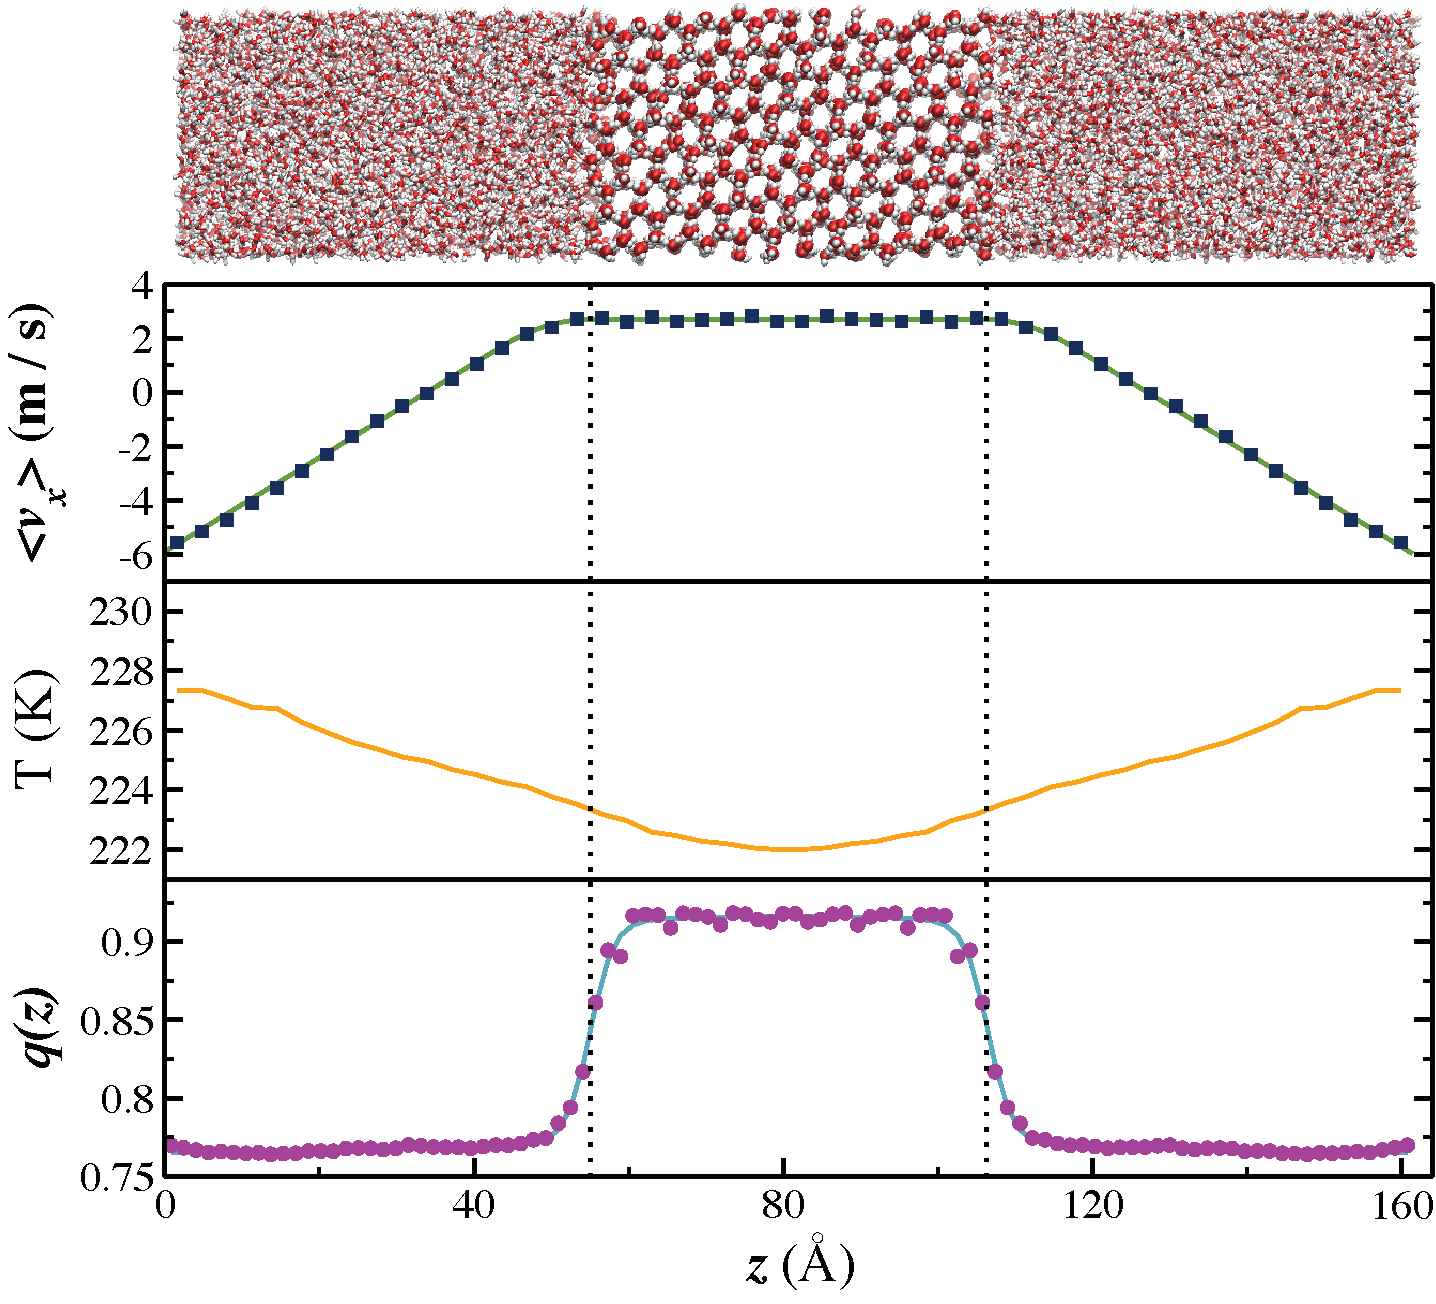
\includegraphics[width=\linewidth]{Figures/SecPrismComicStrip}
\caption{\label{fig:spComic} Properties of the secondary prism
  interface (top) being sheared through water at 8.6 m
  s\textsuperscript{-1}. Lower panel: the local tetrahedral order
  parameter, $q(z)$, (circles) and the hyperbolic tangent fit
  (turquoise line).  Middle panel: the imposed thermal gradient
  required to maintain a fixed interfacial temperature of $\sim$225 K
  with the SPC/E water model. Upper panel: the transverse velocity
  gradient (squares) that develops in response to an imposed momentum
  flux, along with the fit (green line). The vertical dotted lines
  indicate the locations of the Gibbs dividing surfaces of the two
  interfaces.}
\end{figure}

In the middle panel of Fig. \ref{fig:spComic}, we show the resulting
thermal gradient from the imposed kinetic energy flux. For the SPC/E
water model, the interfacial temperature is held at $\sim$ 225~K
(270~K for the TIP4P/Ice), allowing investigation of the response to
the shear while maintaining solid / liquid coexistence. In the top
panel, the velocity gradient resulting from the imposed momentum flux
shows that the ice has a uniform positive velocity along the $x$
axis. The bulk liquid at the ends of the simulation cell has negative
velocity, although the center of mass of the simulation box is
stationary.  The bulk fluid shows a primarily linear velocity gradient
allowing for easy calculation of the shear viscosity using
Eq. \eqref{eq:viscosity}. Close to the interface, the ice imparts
significant positive momentum into the surrounding interfacial liquid.
Projections of the velocity gradient from the liquid onto the Gibbs
dividing surface indicate that the ice-water interface is in the
negative slip regime.

From Eq. \eqref{tet_fit}, we have obtained estimates for $w$, the
structural widths of the interfaces for the quiescent ice / water
systems. These values are related to the $10\%-90\%$ interfacial
widths commonly reported in previous studies
($w_\mathrm{10-90} = 2.197~w$).\cite{Bryk2002,Bryk2004} For the SPC/E
interfaces at 225~K, we find $w_\mathrm{10-90} \approx 7$~\AA~ as seen
in Table \ref{tab:propsSPCE}.  These values are similar to our previous
findings for the $10\%-90\%$ interfacial widths obtained from shorter
simulations, ($7.0 \pm 0.9$ \AA) for basal and ($7.9 \pm 0.4$ \AA) for
prismatic interfaces.\cite{Louden2013a} The interfacial widths in
TIP4P/Ice systems indicate slightly broader interfaces, where values of
$w_\mathrm{10-90} \approx 9$~\AA~ are more common. These values are
reported in Table \ref{tab:propsTIP4P}.

Over the range of shear rates investigated,
$\sim 0.5-10.0~\mathrm{~m~s}^{-1}$, we find no significant changes in
the interfacial widths for any of the crystal faces. All values of
$w_\mathrm{10-90}$ obtained from shearing simulations fell inside the
error bars of the values obtained from the quiescent simulations.

\begin{table}[h]
\centering
\caption{Computed properties of the
  ice-I$_\mathrm{h}$ interfaces with SPC/E (225~K)
  water. Dynamic widths ($d_\mathrm{10-90}$ and $j_\mathrm{10-90}$)
  are defined in Eqs. \eqref{tauFit} and the discussion section,
  respectively. Uncertainties in the last digit are indicated with
  parentheses.\label{tab:propsSPCE}} 
\begin{tabular}{r|ccc|c}  
  \toprule
  & \multicolumn{3}{c|}{Interfacial Widths (\AA)} & Surface H-bond density \\
  Interface & $w_\mathrm{10-90}$ &  $d_\mathrm{10-90}$ & $j_\mathrm{10-90}$ & $\rho_{sl}$ (\AA\textsuperscript{-2}) \\ 
  \midrule
  Basal  $\{0001\}$                 & 7.5(4) & 11(2) & 11 & 0.1227(3)  \\
  Prismatic  $\{10\bar{1}0\}$       & 7.2(2) & 10(2) & 12 & 0.2014(5)  \\
  Pyramidal  $\{20\bar{2}1\}$       & 6.6(2) & 11(3) & 13 & 0.0866(3)  \\
  Secondary Prism  $\{11\bar{2}0\}$ & 6.7(2) & 11(3) & 10 & 0.1384(4)  \\ 
  \bottomrule
\end{tabular}
\end{table}

\begin{table}[h]
\centering
\caption{Computed properties of the
  ice-I$_\mathrm{h}$ interfaces with TIP4P/Ice (270~K) water. Uncertainties in the last digit are indicated with
  parentheses. \label{tab:propsTIP4P}}
\begin{tabular}{r|ccc|c}  
  \toprule
  & \multicolumn{3}{c|}{Interfacial Widths (\AA)} & 
                                                    Surface H-bond
                                                    density \\
  Interface & $w_\mathrm{10-90}$ &  $d_\mathrm{10-90}$ & $j_\mathrm{10-90}$ & $\rho_{sl}$ (\AA\textsuperscript{-2}) \\ 
  \midrule
  Basal  $\{0001\}$                 & 8.8(8) & 15(3) & 9   & 0.0749(9)\\
  Prismatic  $\{10\bar{1}0\}$       & 9.0(5) & 15(2) & 13  & 0.141(1) \\
  Pyramidal  $\{20\bar{2}1\}$       & 8.2(5) & 13(1) & 10  & 0.074(1) \\
  Secondary Prism  $\{11\bar{2}0\}$ & 9.4(6) & 14(2)   & 12  & 0.119(1) \\
  \bottomrule
\end{tabular}
\end{table}

These values agree reasonably well with those reported by Haymet
\textit{et
  al.}.\cite{Karim1988,Karim1990,Hayward2001,Bryk2002,Hayward2002,Bryk2004}
Using a variety of water models and several different order
parameters, they have estimated the ice / water interface to be
between $5$~\AA~and $18$~\AA~depending on the particular interface and
means of measure.  For the SPC/E model, they found the basal and
prismatic ice / water interface to be $\approx 11$~\AA~ wide from
translational and window-averaged density order parameters. The
interfacial widths were also estimated by observing the transition of
a similar tetrahedral order parameter from their ice-like value of
$0.9$ to the bulk liquid value of $0.6$. This gave estimates of
$\approx 11$~\AA~, somewhat larger than our current estimates. More
careful analysis will be necessary to determine if the proton striped
surface configurations used here are the origin of this discrepancy.

\subsection{Solid / liquid friction at ice / water interfaces}
In no-stick boundary conditions, fluid flowing over a solid is
characterized by a slip length, $\delta$, describing the extent of
slip of the fluid at the interface. This length is the extrapolated
distance from the interface where the tangential velocity component
vanishes. For solids with weak interactions with the liquid, there is
little drag imposed on the fluid and the resulting interfacial liquid
velocity, $\Delta v_\mathrm{slip}$, can be significant. In no-stick
boundaries, therefore, the extrapolated slip lengths are also large
(top panel of Fig. \ref{fig:slipLengthPlot}).  Balasubramanian and
Mundy have related the slip length to the interfacial friction
coefficient, 
\begin{equation}\label{kappa1}
\lambda = \frac{\eta}{\delta}
\end{equation}
where $\eta$ is the shear viscosity of the
liquid.\cite{Balasubramanian1999}

For solids that have strong interactions with the liquid, a larger
frictional drag is imposed on the fluid at the interface and the
resulting slip lengths are smaller. When the solid / liquid interactions
become large enough, the interface is best described with stick
boundary conditions, and the slip length will vanish (middle panel of
Fig. \ref{fig:slipLengthPlot}).  Stick boundaries pose a problem for
Eq.  \eqref{kappa1}, as $\lambda$ asymptotically goes to infinity as
$\delta \rightarrow 0$.  Likewise, some materials possess solid / liquid
interactions that are strong enough for the extrapolated tangential
velocity to vanish \textit{before} reaching the solid. The velocity
profile yields a negative slip length (bottom panel of Fig.
\ref{fig:slipLengthPlot}), and the solid / liquid friction coefficient
defined in Eq. \eqref{kappa1} becomes meaningless.  Ice shearing
through liquid water is in the negative slip limit. The tangential
velocity profile of the liquid extrapolates to the solid velocity
several molecular layers before reaching the solid. Thus a new
friction coefficient must be defined to describe these interfaces.

\begin{figure}
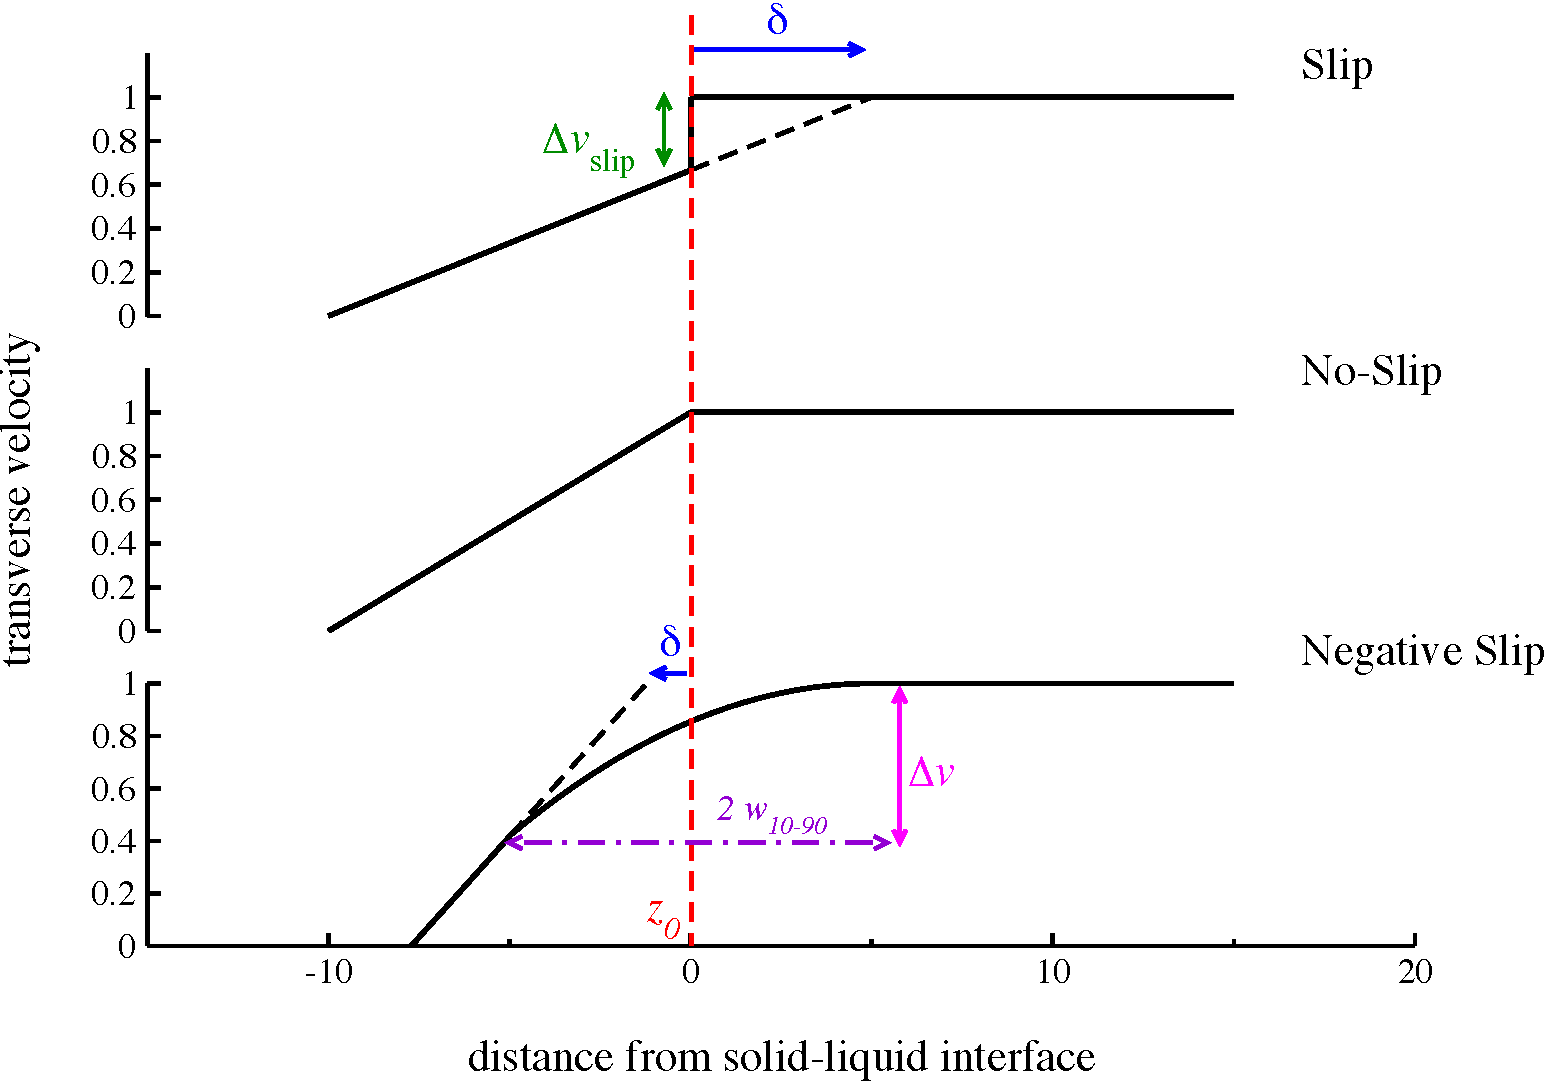
\includegraphics[width=\linewidth]{Figures/slipLengthPlot}
\caption{\label{fig:slipLength} A sketch of transverse velocity
  profiles, $v_x(z)$, for interfaces in slip (top), no-slip (middle),
  and negative slip boundary conditions (bottom).  The location of the
  interface is defined by a Gibbs dividing surface at $z_0$. Under
  negative slip conditions, the 10-90 interfacial width, $w_{10-90}$,
  provides locations that are unambiguously on the liquid and solid
  sides of the interface.\label{fig:slipLengthPlot}}
\end{figure}

A solid / liquid friction coefficient, $\kappa$, may also be defined
using the velocity drop across the interface, rather than the length
scale over which this drop occurs. We can relate the imposed shear
stress with the relative tangential velocity of the fluid in the
interfacial region,\cite{Kuang2012}
\begin{equation}\label{Shenyu-13}
j_{z}(p_{x}) = \kappa_{x} \Delta v
\end{equation}
where $\Delta v = v_{x}(\mathrm{solid}) - v_{x}(\mathrm{liquid})$ is
the difference in transverse velocity between points that are
unambiguously on the solid and liquid sides of the interface.  In slip
boundary conditions, $\kappa$ and $\lambda$ are identical, but
Eq. \eqref{Shenyu-13} provides a direct analogy to non-equilibrium
expressions for the interfacial thermal conductance $(G)$,
\begin{equation}
J_z = G~ \Delta T.
\end{equation}
Here, $J_z$ is a thermal flux and the temperature drop is measured
across an interface of \textit{finite width}. By analogy, $\kappa$ is
a transport coefficient that measures \textit{interfacial momentum
  conductance} across an interface of finite width.

In ice / water interfaces, the solid / liquid boundary is not
an infinitely thin plane. An order parameter (the tetrahedrality) goes
smoothly between the phases over a few molecular diameters.  We can
use this order parameter to find the interfacial width and define
locations in space that are unambiguously on the solid and liquid
sides of the interface.  In what follows, we have used the Gibbs
dividing surface ($z_0$) and the 10$-$90 width of the interface
($w_\mathrm{10-90}$) to arrive at physical locations for measuring
$v_{x}(solid)$ and $v_{x}(liquid)$.  These uniquely define a friction
coefficient in terms of well-defined structural features ($z_0$ and
$w_\mathrm{10-90}$) and dynamic properties ($v_{x}(z)$) of the
interface.

Tangential velocity profiles from the simulations were fit using a
piecewise function that is both continuous and continuously
differentiable (see Supporting Information). To arrive at estimates of
the interfacial velocities, these fits were queried at locations on
either side of the structural Gibbs dividing surface,
\begin{align}
v_{x}(\mathrm{solid}) & = v_{x}( z_0 + w_\mathrm{10-90})  \label{eq:vx1}\\
v_{x}(\mathrm{liquid}) & = v_{x}( z_0 - w_\mathrm{10-90}). \label{eq:vx2}
\end{align}
The momentum flux, $j_{z}(p_{x})$ is an imposed parameter of the
VSS-RNEMD simulations, and by using Eq. \eqref{Shenyu-13}, estimates
of interfacial friction coefficient $\kappa$ are straightforward.

The calculated $\kappa$ values found for the four crystalline facets
of ice-I$_\mathrm{h}$ investigated here are shown in Table
\ref{tab:kappa}. Solid / liquid friction coefficients for shearing
simulations where the imposed momentum flux was in the $y$-dimension,
$\kappa_{y}$, are calculated in the same manner, with $j_{z}(p_{y})$
and $v_{y}$ substituting for $j_{z}(p_{x})$ and $v_{x}$ in
Eqs. \eqref{Shenyu-13}, \eqref{eq:vx1}, and \eqref{eq:vx2}.  These
results were found to be independent of the shear rate (see Fig. S8
in the Supporting Information), as well as the direction of the shear
relative to the features on the surfaces of the facets.

\begin{table}[h]
\centering
\caption{Solid / liquid friction coefficients (in units of amu \AA\textsuperscript{-2} fs\textsuperscript{-1}) for
  ice-I$_\mathrm{h}$ interfaces with water. Uncertainties in the last digit are indicated with
  parentheses.\label{tab:kappa}}
\begin{tabular}{r|cc|cc}  
  \toprule
  & \multicolumn{2}{c|}{SPC/E (225~K)} & \multicolumn{2}{c}{TIP4P/Ice (270~K)} \\
  Interface & $\kappa_{x}$ &  $\kappa_{y}$ & $\kappa_{x}$ &  $\kappa_{y}$ \\ 
  \midrule
  Basal  $\{0001\}$                 & 0.32(5)  & 0.31(4) & 0.12(2)  & 0.13(2) \\
  Prismatic  $\{10\bar{1}0\}$       & 0.44(5)  & 0.46(5) & 0.16(2)  & 0.16(3) \\
  Pyramidal  $\{20\bar{2}1\}$       & 0.28(3)  & 0.25(3) & 0.09(1)  & 0.10(1) \\
  Secondary Prism  $\{11\bar{2}0\}$ & 0.44(4)  & 0.42(5) & 0.14(3)  & 0.14(2) \\ 
  \bottomrule
\end{tabular}
\end{table}

Note that the values of $\kappa$ for the basal and prismatic crystal
facets in Table \ref{tab:kappa} disagree with values for interfacial
friction ($\lambda$) we previously reported.\cite{Louden2013a} In our
initial report, the expression for the coefficient of friction was
derived from equation \eqref{kappa1} and the linear constitutive
relation for shear stress in a bulk fluid.  However, as described
above, sheared ice / water interfaces are in the domain negative slip
lengths. Eq. \eqref{kappa1} should only be used in slip boundary
conditions, as negative slip can yield coefficients of friction that
appear to be smaller in magnitude than the zero slip conditions. In
our previous work, the prismatic surface was found to have a larger
negative slip length than the basal face, indicating a prismatic
surface that should have been reported with a larger coefficient of
friction. If one instead uses Eq. \eqref{Shenyu-13} and interfacial
widths to compute friction, the reported values come into agreement.

The two water models give two significantly different values for the
friction coefficients. This is primarily a result of the difference in
water viscosities at the two coexistence temperatures ($\eta = $ 15.9
cP for SPC/E at 225K and 6.1 cP for TIP4P/Ice at 270K), which alters
the stream velocity on the liquid side of the interface. The relative
ratios of facet friction are similar in both models, however, with
$\kappa_\mathrm{prismatic} / \kappa_\mathrm{basal} =$ 1.56~(SPC/E) and
1.32~(TIP4P/Ice),
$\kappa_\mathrm{pyramidal} / \kappa_\mathrm{basal} =$ 0.84~(SPC/E) and
0.81~(TIP4P/Ice), and
$\kappa_\mathrm{secondary} / \kappa_\mathrm{basal} =$ 1.33~(SPC/E) and
1.15~(TIP4P/Ice). The observed ordering of facet friction
coefficients,
\begin{equation}
\kappa_\mathrm{pyramidal} < \kappa_\mathrm{basal} <
\kappa_\mathrm{secondary} < \kappa_\mathrm{prismatic} 
\end{equation} 
seems robust.

\subsection{Dynamic measures of interfacial width under shear}
The spatially-resolved orientational time correlation function,
\begin{equation}\label{C(t)1}
  C_{2}(z,t)=\langle P_{2}(\mathbf{u}_i(0)\cdot \mathbf{u}_i(t))
  \delta(z_i(0) - z) \rangle,
\end{equation}
provides local information about the decorrelation of molecular
orientations in time. Here, $P_{2}$ is the second-order Legendre
polynomial, and $\mathbf{u}_i$ is the molecular unit vector that bisects
the HOH angle of molecule $i$. The angle brackets indicate an average
over all the water molecules and time origins, and the delta function
restricts the average to specific regions in the $z$-dimension. 

In the ice crystal, decay of $C_2(z,t)$ is incomplete, while in the
liquid, correlation times are typically measured in ps. Observing the
spatial transition between the decay regimes can define a dynamic
measure of the interfacial width. To determine dynamic widths of the
interfaces under shear, each of the systems were divided into bins
along the $z$ axis ($\approx$ 1 \AA\ wide) and $C_2(z,t)$ was computed
using only those molecules that were in the bin at the initial
time. For each ice / water interface investigated, the following 0.5
ns simulations were computed: quiescent simulations (where no thermal
or momentum gradient was present), simulations with only a thermal
gradient present, and simulations where both thermal and momentum
gradients were present. During these simulations, the positions and
orientations of each molecule were recorded every 100 fs.

\begin{figure}
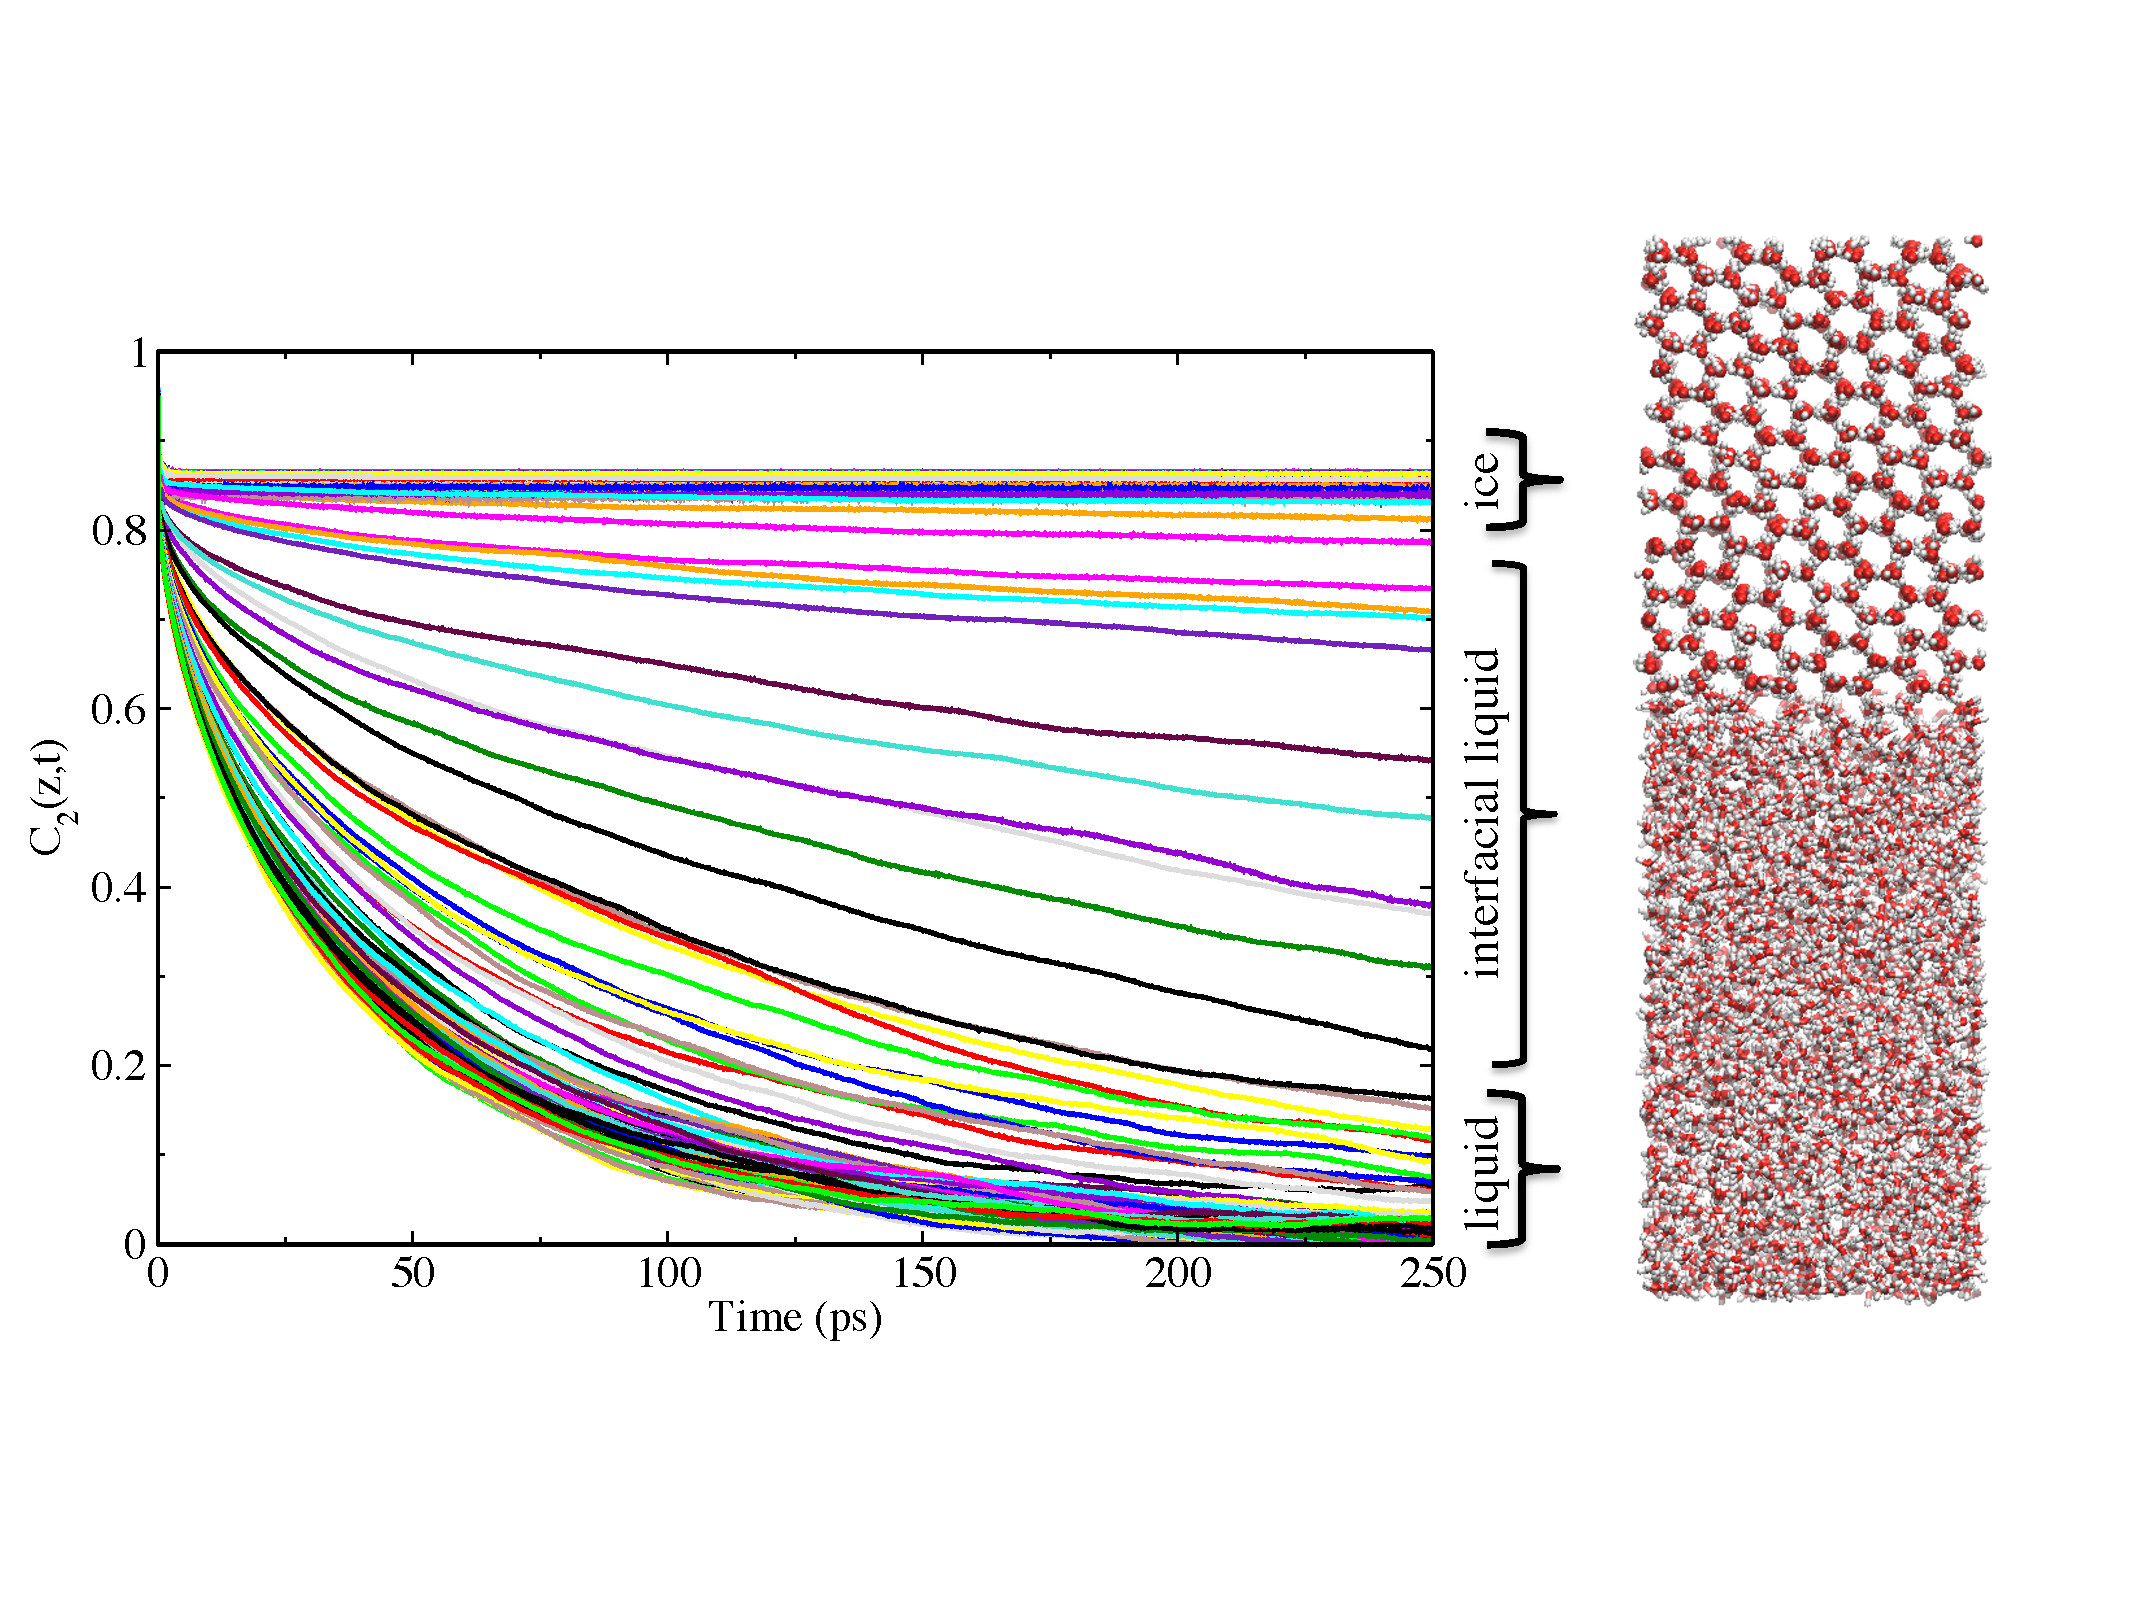
\includegraphics[width=\linewidth]{Figures/CztImage}
\caption{\label{fig:Czt} $C_2(z,t)$ collected in 1 \AA~bins across the SPC/E
  secondary prism ice / water interface. The band that experiences very
  little decay represents water molecules in the ice, while the band
  that decays quickly corresponds to bins in the liquid.  The
  correlation function presents a continuous distribution of decay
  behaviors across the interface between ice and liquid water.}
\end{figure}

Recently, Laage and Hynes have determined the mechanism for water
reorientation.\cite{Laage2006,Laage2008} Using molecular dynamics
simulations, they found that water reorients by breaking a hydrogen
bond with an overcoordinated first-shell neighbor, and makes a large
angle jump to form a new hydrogen bond with an undercoordinated
second-shell neighbor. The hydrogen bond cleavage and molecular
reorientation occur in a concerted fashion, not in successive steps as
was previously thought. With this detailed picture, they constructed
the Extended Jump Model\cite{Laage2006,Laage2008} based on the Ivanov
Jump Model and parameters extracted from their molecular simulations;
the average jump amplitude of the rotational jump, $\theta_{0}$, and
the frequency of the jumps, $1/\tau_{0}$. After accounting for
molecular frame reorientation, the Extended Jump Model is able to
predict reorientation relaxation times, $\tau_{n}^{jump}$, which agree
with experimental results as well as estimates obtained from
simulations where fast librational motion is ignored.

Computed $C_2(z,t)$ values have previously been fit to a
triexponential decay, with three time constants:
$\tau_\mathrm{short}$, measuring the librational motion of the water
molecules, $\tau_\mathrm{middle}$, measuring the timescale for the
large angle jumps during the breaking and making of hydrogen bonds,
and $\tau_\mathrm{long}$, corresponding to the translational motion of
the water molecules.\cite{Louden2013a} The Extended Jump Model also
includes three similar decay constants, however two of them are linked
and the dynamics of the decay is governed by two parameters. Since we
are interested in how the decay times and the individual contributions
may change through the interface, we have fit the $C_2(z,t)$ data
with
\begin{equation}
  C_{2}(z,t) = a~e^{-t/\tau_\mathrm{short}} + b~e^{-t/\tau_\mathrm{middle}} + 
  (1-a-b)~e^{-t/\tau_\mathrm{long}}
\label{eq:c2}
\end{equation}
where all of the decay constants are considered local functions of the
$z$ coordinate. In Fig. \ref{fig:SPorient}, the $z$-coordinate
profiles for the three decay constants, $\tau_{\mathrm{short}}$,
$\tau_{\mathrm{middle}}$, and $\tau_{\mathrm{long}}$ for the secondary prism interface
is shown, along with their fractional components of the overall total
decay, ($a$, $b$, $1-a-b$), respectively. Similar figures for the
other interfaces are provided in the Supporting Information.

In the liquid regions of all four interfaces, $\tau_\mathrm{middle}$
and $\tau_\mathrm{long}$ consistently approach $3-6$ ps and $30-40$
ps, respectively.  Both of these times increase closer to the
interface.  Conversely, $\tau_\mathrm{short}$ decreases from a
liquid-state value of $72-76$ fs approaching the interface.

The fractional contributions of the three motions to the overall decay
changes as we approach the interface as well. Far from the ice, the
librational motion and hydrogen bond breaking/making events each
contribute to about 20 percent of the total decay, whereas frame
reorientation contributes about 60 percent. As we approach the
interface, the librations and hydrogen bond dynamics both decrease in
contribution. The librations comprise approximately 15 percent of the
overall decay at the edge of the interface, whereas the hydrogen bond
contributions drop to approximately zero. In contrast, the fraction of
the total decay due to frame reorientation is shown to increase
approaching the interface.  The time constant corresponding to this
motion is seen to logarithmically increase as we approach the interface
as the molecules become more ice-like. In the ice we would expect
molecular reorientation to be incomplete, however, at the interface we
observe frame reorientation to contribute 85 percent of the overall
decay.

\newpage
\begin{figure}
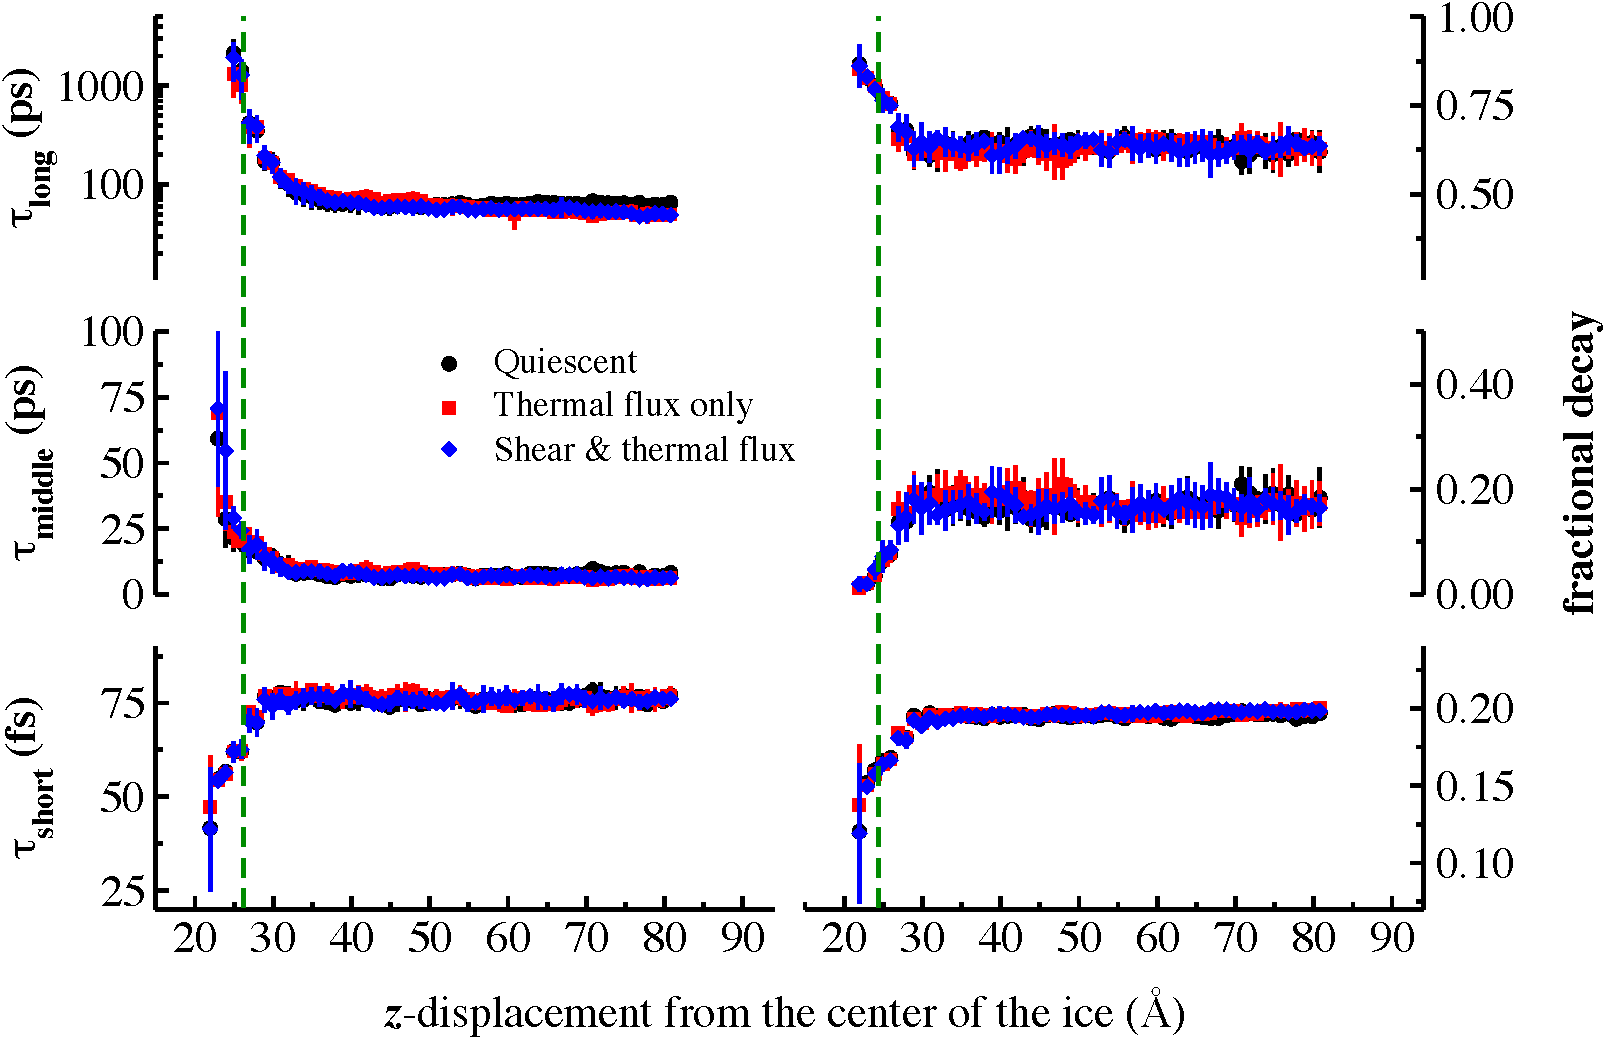
\includegraphics[width=\linewidth]{Figures/Sec_lcorrz}
\caption{\label{fig:SPorient} Decay times (left) for $C_2(z,t)$ at the
  SPC/E secondary prism interface, and their fractional contributions to the
  overall decay (right) fit using Eq. \eqref{eq:c2}. The local decay
  constants are plotted as a function of distance from the center of
  the ice slab. The vertical dashed line indicates the Gibbs dividing
  surface determined using the local tetrahedral order parameter.
  Results are shown for a quiescent system with no applied kinetic or
  momentum flux (black), an interface with an imposed
  kinetic energy flux (red), and a sheared simulation (blue) with both
  kinetic and momentum fluxes.}
\end{figure}

The middle and long decay times diverge inside the ice crystal, so the
orientational rate, $k(z) = 1 / \tau(z)$ can be used to identify a
dynamic interfacial width for the interface by fitting the profiles of
the middle and long-time orientational rates with a function that goes
smoothly between bulk-like liquid behavior and the crystal,
\begin{equation}\label{tauFit}
  k(z) = \frac{1}{\tau_\mathrm{liquid}} - \frac{1}{2~\tau_\mathrm{liquid}} \left(
      \tanh \left( \frac{z-l}{d} \right) - \tanh \left( \frac{z-r}{d} \right) \right)
\end{equation}
where $l$ and $r$ are the locations of the Gibbs dividing surfaces,
and $d$ is a dynamic width.  As with the structural widths,
$10\%-90\%$ dynamic widths are easily computed from the fits
($d_\mathrm{10-90} = 2.197~d$).  These values are provided in Tables
\ref{tab:propsSPCE} and \ref{tab:propsTIP4P}. All four SPC/E
interfaces exhibit dynamic widths that are $\sim 11$~\AA, and are
larger than the structural widths computed above.  In TIP4P/Ice at
270K, the dynamic widths are $\sim 14$~\AA, also larger than the
structural widths in for these interafaces.

We note that Bryk and Haymet also calculated the orientational time
correlation function at the basal interface of SPC/E
water,\cite{Bryk2002} and observed the same qualitative trend through
the ice / water interface, although the spatial resolution was not
sufficient to resolve a dynamic width.
 
\section{Discussion}
The primary result of this paper is the observation that the different
facets of ice-I$_\mathrm{h}$ produce significantly different solid /
liquid interfacial friction coefficients with water (see Table
\ref{tab:kappa}).  The two prismatic surfaces displayed the largest
coefficients of friction, while the basal and pyramidal facets
exhibited significantly lower friction. This trend is robust over a
wide range of shear rates, and shear direction relative to ice surface
features. Also, while the magnitude of the solid / liquid friction
coefficients differ due to liquid viscosities, the facet trends are
exhibited by both SPC/E and TIP4P/Ice at their coexistence
temperatures.

It is surprising that the observed solid / liquid friction
coefficients do not depend on the shear direction relative to surface
features. Pfalzgraff \textit{et al.} have recently investigated
diffusion of the water molecules comprising the QLL on the vacuum
exposed basal, prismatic, and pyramidal surfaces of an
ice-I$_\mathrm{h}$ crystal.\cite{Pfalzgraff2011} They observed
anisotropic diffusion on the prismatic and pyramidal surfaces at 250~K
with the NE6 model ($\sim$~40~K below the melting temperature of that
model). In two following studies, Gladich \textit{et al.}
investigated the temperature dependence of this phenomena and deduced
the mechanism of anisotropic self-diffusivity at the prismatic
ice-vapor interface.\cite{Gladich2011,Gladich2015} They observed a
transition from anisotropic to isotropic diffusion at about 260~K with
the NE6 model, and attributed the transition to a change in the
prevailing mechanism of self-diffusion. At temperatures colder than
260~K, the QLL is sparse and the diffusing molecules are strongly
influenced by the underlying geometry of the crystal. At temperatures
warmer than 260~K, the QLL is thicker and diffusion occurs at the
outer part of the QLL. These results were robust for TIP4P/2005 and
TIP5P-Ew at the same relative undercooling temperature. Since our ice
/ water interfaces are at their respective coexistence temperatures,
the effects of the underlying ice crystal may be masked and we might
expect to recover isotropic behavior.

The differences in friction are also surprising given that densities
and molecular interactions are identical for the four interfaces and
the interfacial widths measured via both structural and dynamic
features are also quite similar (for the interfaces treated with the
same water model). There are few remaining surface properties that
could give rise to differences in solid / liquid friction of the four
facets, notably surface corrugation, hydrogen bonding density, and
hydrogen bond lifetime at the interface. In this section we
investigate the roles of these surface features.

\subsubsection{Solid / liquid hydrogen bond density}
The four ice surfaces may potentially have different densities of
hydrogen bonds that bridge the solid and liquid. An ice surface that
forms more hydrogen bonds with the interfacial liquid would be able to
exert significant lateral forces on the liquid layer, yielding a
larger friction coefficient. To probe this possibility, we have
investigated the density of cross hydrogen bonds between the ice and
the liquid.

Quantifying water molecules as ``ice'' or ``liquid'' at an interface
of finite width requires a local order parameter for separating the
molecules.  Conde \textit{et al.}\cite{Conde2008} (and later Gladich
\textit{et al.}\cite{Gladich2011,Gladich2015}) discriminated molecules
as either ``ice'' or ``liquid'' by a threshold value of the local
tetrahedral order parameter (the same order parameter described here
in section \ref{structure}), denoted $q_{t}$. This threshold value was
obtained by equating the probability of incorrectly assigning a
liquid-like molecule as ice-like to the probability of incorrectly
assigning an ice-like molecule as liquid-like. Molecules with
$q < q_{t}$ were denoted as liquid-like, while those found having
$q > q_{t}$ were designated ice-like.

In a similar manner, we have chosen a threshold value of the local
tetrahedral order parameter as our partitioning criterion. Here,
$q_{t}$ is taken to be the value of the order parameter at the Gibbs
dividing surface ($q(z_0) \approx 0.84$ for SPC/E and
$q(z_0) \approx 0.85$ for TIP4P/Ice).  Note that some molecules have
strong tetrahedral ordering in the liquid phase, so this segregation
will not yield perfect division between ice and liquid phase
molecules.

To determine if a hydrogen bond has been formed between two water
molecules, we used the geometric criteria of Luzar and
Chandler.\cite{Luzar1996} We identify a hydrogen bond between two
water molecules if the distance between their oxygen sites,
$r_\mathrm{OO} < 3.5$~\AA, and the OHO bond angle,
$\theta_\mathrm{OHO} < 30^\circ$.

For each of the shearing simulations performed above, a hydrogen bond
tetrahedrality matrix was constructed.  Snapshots from the shearing
trajectories were taken every $0.1$ ps, and the tetrahedrality $(q)$
value for each water molecule in the system was calculated. Hydrogen
bonds were also identified, and the tetrahedrality of the donor
$(q_{D})$ and acceptor $(q_{A})$ molecules were recorded. A
probability density of hydrogen bonds categorized by donor and
acceptor tetrahedrality, $\rho_\mathrm{HB}(q_D, q_A)$, was then
recorded.

\begin{figure}
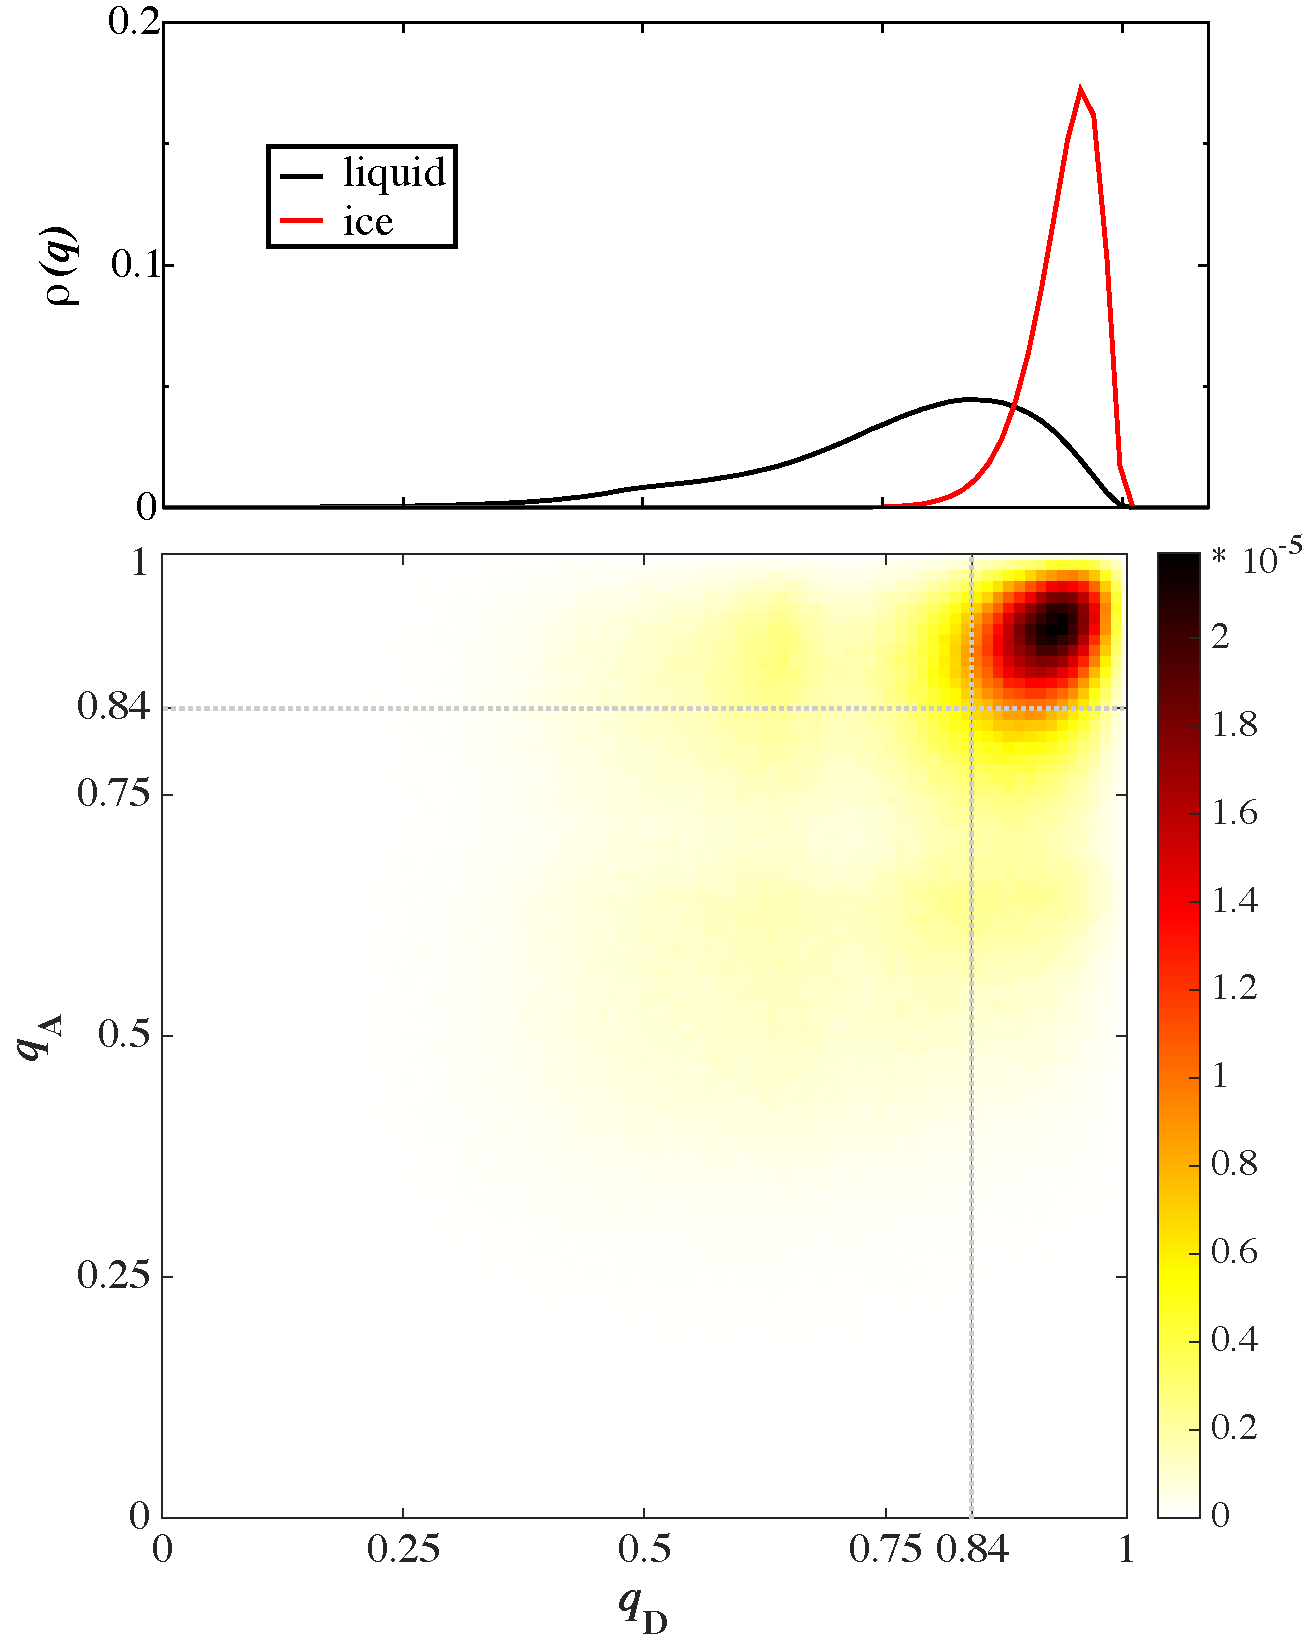
\includegraphics[width=5in]{Figures/hbtet.pdf}
\caption{\label{fig:tetHBMatrix} Distribution of hydrogen bonds at a
  prismatic interface showing the tetrahedralities of donor $(q_D)$
  and acceptor $(q_A)$ molecules (lower panel). Distributions of
  tetrahedralities in bulk ice and liquid phases are shown in the
  upper panel. The value of $q$ at the Gibbs dividing surface is
  indicated with dashed lines. Hydrogen bonds between ice molecules
  are represented by the upper right square, while those between
  liquid molecules are in the lower left.  Hydrogen bonds that bridge
  the ice-liquid interface exist primarily in the vertical and
  horizontal strips that remain.}
\end{figure}

The lower panel of Fig. \ref{fig:tetHBMatrix} shows a hydrogen bond
tetrahedrality distribution for the prismatic facet with $q_{D}$
plotted along the $x$-axis and $q_{A}$ along the $y$-axis.  Population
around $q_{D} \approx q_{A} \approx 0.9$ indicates the density of
ice-ice hydrogen bonds in the system, while the liquid-state hydrogen
bonds are concentrated in the lower left, and are significantly more
diffuse.  The off-diagonal regions of the distribution represent the
population of molecules in tetrahedral (ice-like) environments bound
to non-tetrahedral (liquid-like) environments. Integrating the
population found in each of these regions and normalizing by the
surface area of each ice crystal produces a surface density of
hydrogen bonds (\AA\textsuperscript{-2}) formed between the ice and
interfacial liquid,
\begin{equation}\label{hbondDensity}
\rho_{sl} = \frac{N_\mathrm{HB}}{2 L_{x}L_{y}} \left[ \int_0^{q_{t}}
  dq_{D} \int_{q_{t}}^1 dq_{A}~\rho_\mathrm{HB}(q_{D},q_{A}) +  \int_0^{q_{t}}
  dq_{A} \int_{q_{t}}^1 dq_{D}~\rho_\mathrm{HB}(q_{D},q_{A}) \right]
\end{equation}
$N_\mathrm{HB}$ is the total number of hydrogen bonds found in the
system, and $L_x$ and $L_y$ are the dimensions of the two ice facets
exposed to the liquid.  Values for $\rho_{sl}$ for each of the ice
surfaces are reported in Table \ref{tab:kappa}.

The trend in surface density of solid / liquid hydrogen bonds
reproduces the trend in the friction coefficients, indicating that
friction at ice-I$_\mathrm{h}$ water interfaces is strongly influenced
by the number of solid / liquid hydrogen bonds that can be formed.
This result is robust under multiple shear rates and orientation of
shear flow relative to the surface features of the ice (that is, shear
in both the $x$ and $y$ dimensions), indicating that the hydrogen
bonding statistics between an ice facet and the liquid are not altered
by the imposed shear.

\subsubsection{Surface corrugation}
A second possible influence on the friction coefficient is the surface
topography of the ice crystals. To investigate this possibility, we
computed the mean projected density ($\rho(y,z)$) for each of the
ice / water systems; details of these computations can be found in the
Supplemental Information. The structure of the surface corrugation can
be obtained by measuring the peak-to-peak distances of the
liquid-exposed crystal structures, the dimensions of which are
reported in Table \ref{tab:surf}. When a crystal of ice-I$_\mathrm{h}$
is cleaved along either of the two prismatic crystal facets, the
exposed oxygen atoms present channel-like structures with channel
widths of $\sim$ 5~\AA~ and channel depths of $\sim$ 2.3~\AA~.  When
cleaved along the pyramidal facet, the resulting surface features a
much larger channel, $\sim$ 8.3~\AA~ wide.  Conversely, the basal
surface presents a rather smooth surface to the liquid, with stripes
of oxygen atoms forming surface ripples with depths of $\sim$ 1~\AA~.

\begin{table}[h]
\centering
\caption{Surface features of Ice-I$_\mathrm{h}$ facets.\label{tab:surf}}
\begin{tabular}{r|cc}  
\toprule
Interface & Channel width (\AA) & Channel depth (\AA) \\ 
\midrule
Basal  $\{0001\}$                 & 3.5(2) & 0.9(1)  \\
Prismatic  $\{10\bar{1}0\}$       & 4.5(1) & 2.4(3)  \\
Pyramidal  $\{20\bar{2}1\}$       & 8.3(2) & 1.9(4)  \\
Secondary Prism  $\{11\bar{2}0\}$ & 5.3(4) & 2.2(1)  \\ 
\bottomrule
\end{tabular}
\end{table}

The prismatic channels are quite stable. That is, the projected
density in the prismatic and secondary prism surface channels is small
relative to the bulk liquid density $(\rho(y,z) < \rho_l / 7)$.  One
might expect regions of low liquid density to yield smaller solid /
liquid interactions, and it does appear that these two surfaces
present roughly half of the surface oxygen atoms to the liquid.
However, the molecules forming the bottoms of the channels are fully
saturated (four hydrogen bonds each), while the molecules that form
the tops of the channels present a high density of available hydrogen
bond locations.

The oxygen-based surface features of the prism and secondary prism are
similar, and only the orientation of the water molecules varies.  This
means that the patterning of donor and acceptors on the two facets is
quite different. A liquid with internal hydrogen bonding constraints
that is in contact with these facets will allow the prismatic surface
to form a higher density of solid / liquid hydrogen bonds than the
secondary prism, even with identical oxygen ordering at the interface.

% In contrast with the prismatic facets, liquid state molecules can
% populate the surface channels on the pyramidal facet. Again, one might
% expect the interactions between the solid and the liquid in close
% physical contact to be quite large.  However, the liquid molecules
% populating this channel do not pack efficiently and cannot fully
% saturate the surface locations available for hydrogen bonding,
% resulting in a lower solid / liquid hydrogen bond density and a
% smaller coefficient of friction.

With its smooth surface, one could make reasonable physical arguments
for the basal face to have either high or low friction with liquid
water. That is, liquid molecules should be able to form a fully
populated network of hydrogen bonds with the surface, as there are no
recessed surface molecules at the bottoms of deep channels. In the
absence of large surface undulations, however, liquid-phase molecules
should also be able to slip over the surface easily. However, the
basal facet was found to have an intermediate friction coefficient
compared with the other facets studied here. The sensible explanation
in light of the hydrogen bonding data is simply that the surface
density of solid / liquid hydrogen bonds (however transitory)
dominates the interfacial friction.

\subsubsection{Spatial resolution of Hydrogen bond jump rates}
The spatially-resolved hydrogen bond jump correlation function,
\begin{equation}\label{jump}
C_\mathrm{jump}(z,t) = 1 - \langle n_a(0) n_b(t) \delta(z_i(0) - z) \rangle
\end{equation}
measures the decorrelation of a hydrogen bond on molecule $i$ as it
transitions between one acceptor ($a$) and another ($b$). $n_a(0)$ is
set to one if hydrogen $i$ is bound to acceptor $a$ at time $0$, and
is zero otherwise.  Absorbing boundaries are utilized with this
correlation function; switches from $b$ back to $a$ at a later time
are considered a new jump, and the angle brackets indicate an average
over all donor hydrogens and time origins. Laage and Hynes determined
the bulk version of this function had \textit{single}-exponential
decay in room temperature water.

A version of this correlation function was used to investigate how
water molecules reorient around
ions\cite{Laage2007,Laage2008a,Stirnemann2011a,Laage2011},
proteins\cite{Duboue-Dijon2014}, and in confined
spaces\cite{Laage2012b,Fogarty2014}.  Laage and Hynes studied how the
strength of the hydrogen bond might perturb the reorientation
dynamics,\cite{Laage2006a} and found the librational motion which
forms a cone around the O-O vector is smaller for more strongly
hydrogen bonded water. This may also provide a partial explanation for
the increasing contribution of short time orientational decay very
close to the ice surfaces.  Since the solid creates an excluded volume
for the water molecules that are in proximity to the interface, the
hindered range of motion (i.e., a smaller cone around the O-O vector)
manifests as faster librational decay.

As an additional measure of a dynamic width of the quiescent
interfaces, each of the systems were divided into bins along the $z$
axis ($\approx$ 1 \AA\ wide) and $C_\mathrm{jump}(z,t)$ was computed.
Like Laage and Hynes, we find that within each spatial region, the
decay is easily fit with a single exponential, yielding a local
hydrogen bond jump time. The jump times diverge inside the ice
crystal, so the jump rate, $k_\mathrm{jump}(z) = 1 / \tau_0(z)$ can be
used to identify a hydrogen bond jump width for the interface in a
similar manner to the dynamic width. $k_\mathrm{jump}(z)$ was fit with
a hyperbolic tangent (see Eq. \eqref{tauFit}) and the 10-90 jump
width, $j_\mathrm{10-90}$, is shown in tables \ref{tab:propsSPCE} and
\ref{tab:propsTIP4P}.

\subsubsection{A simple model for solid-liquid friction}
The interfacial friction coefficient, $\kappa$ captures the momentum
conductance transverse to the interface, and this momentum should be
transferred via strong intermolecular interactions across the
interface. This is measured in ice / water systems by the surface
density of hydrogen bonds, $\rho_\mathrm{s-l}$.  The momentum is then
carried through the liquid via viscous forces $(\eta)$ across an
interfacial region that has width $w_\mathrm{s-l}$. A simple linear
model,
\begin{equation}
  \kappa = c~~\rho_\mathrm{s-l}~~\eta~~w_\mathrm{s-l},
\label{eq:model}
\end{equation}
captures these features at the ice / water interface, and the results
for the two water models nearly coalesce with a proportionality
constant, $c = 0.343$.  The structural width, $w_\mathrm{10-90}$, and
values for $\eta$ for each ice / water system were obtained by fitting
the liquid portions of the simulation box in conjunction with equation
\eqref{eq:viscosity}.  The two water models have two different
coexistence temperatures, so they exhibit different hydrogen bond
densities and viscosities adjacent to the interface.  Comparing
Eq. \eqref{eq:model} with the non-equilibrium expressions for $\kappa$
(Eq. \eqref{Shenyu-13}) and $\eta$ (Eq. \eqref{eq:viscosity}) shows
that the liquid's viscosity is an important feature in capturing the
velocity drop on the liquid side of the interface
($\eta w_\mathrm{s-l}$), but the magnitude of the solid-liquid
interactions ($c~~\rho_\mathrm{s-l}$) plays a central role in the
observed friction.

\begin{figure}
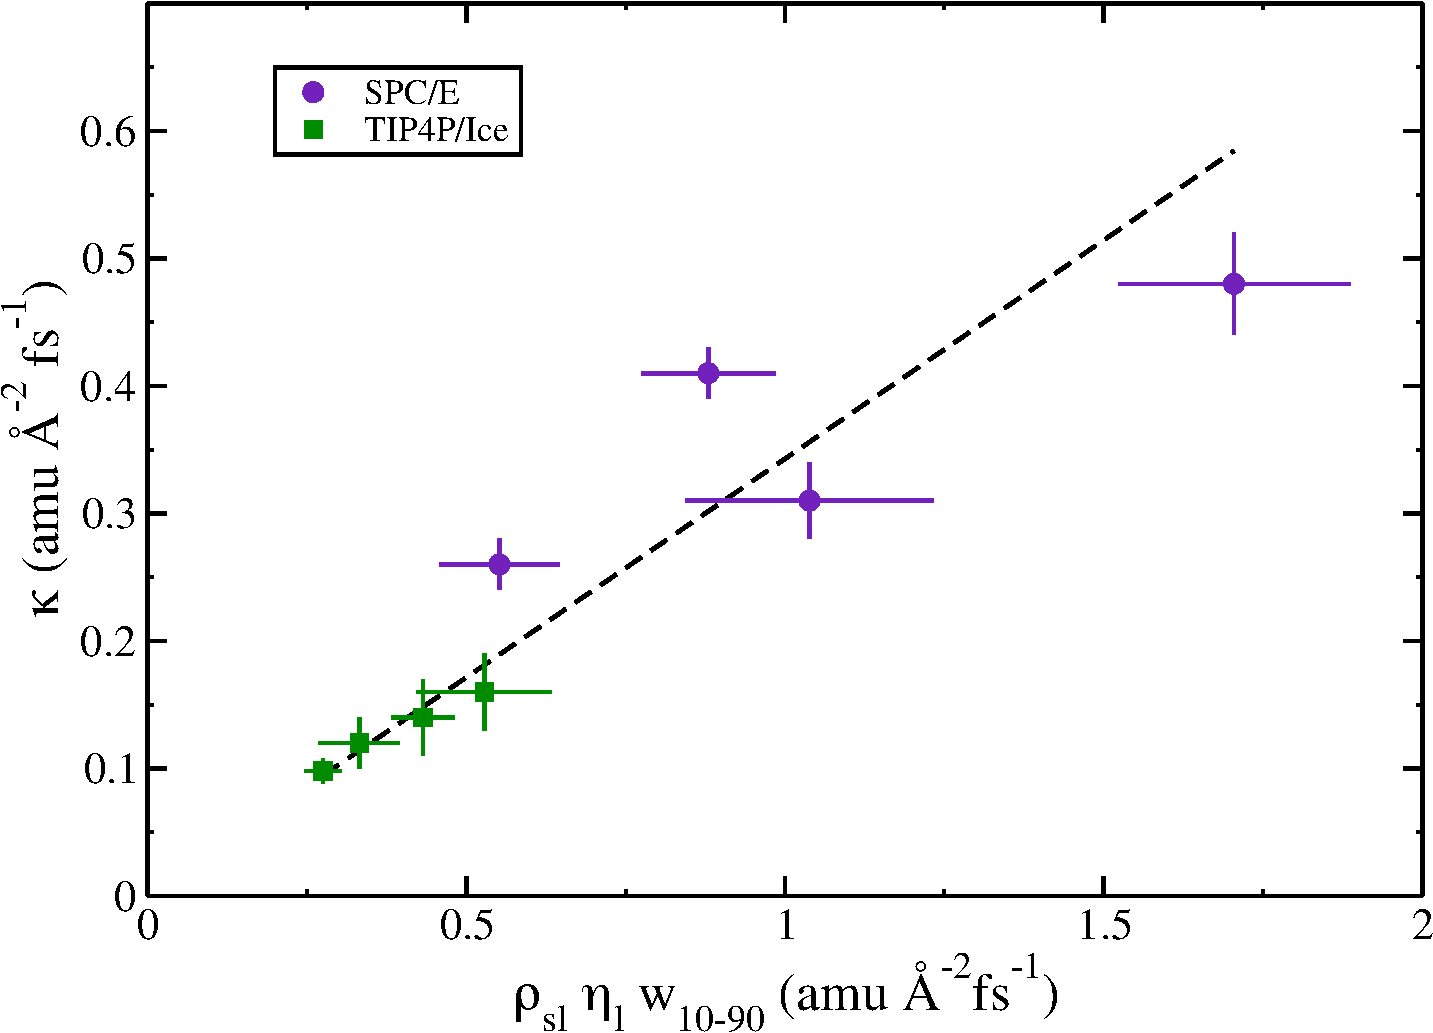
\includegraphics[width=\linewidth]{Figures/simpleModel}
\caption{\label{fig:simpleModel} Solid-liquid friction coefficients
  shown vs. surface hydrogen bond density model (Eq. \eqref{eq:model}
  for all four facets and for both water models.  Although SPC/E
  (225K) and TIP4P/Ice (270K) operate in two distinct viscosity
  domains, the model captures the importance of the density of
  solid-liquid hydrogen bonds.}
\end{figure}                                            

\section{Conclusions}
RNEMD simulations of the different facets of ice being drawn through
surrounding water at the coexistence temperature indicate
facet-dependence of solid / liquid friction.  We have defined a
negative slip interfacial friction coefficient, $\kappa$ (measured in
amu~\AA$^{-2}$ fs$^{-1}$) and find that the two prismatic facets exert
the largest drag on the surrounding liquid.  The basal facet provides
an intermediate level of drag, while the pyramidal facet has roughly
half the interfacial friction of the prismatic facet.

Using the local tetrahedral order parameter as a metric to
differentiate ice and liquid water molecules and a geometric hydrogen
bonding criteria, the friction coefficients were shown to be largely
governed by the surface density of solid / liquid hydrogen bonds
($\rho_{sl}$).  A simple linear model, Eq. \eqref{eq:model}, uses
this density to provide estimates of solid-liquid friction that give
good agrement for two different water models at their respective
coexistence temperatures.

In addition, we have found the ice / water interfacial widths for all
four crystal facets to be similar (using both structural and dynamic
measures) and found these widths to be independent of shear rate.  The
similarity of interfacial width estimates for the four facets indicate
that the particular facet of the exposed ice crystal has very little
effect on how far into the bulk the ice-like structural ordering
persists. While differences have been found in previous simulations of
ice / water interfaces,\cite{Hayward2001,Hayward2002} experimentally
these differences have been less clear.\cite{Beaglehole1993} The
significant differential friction coefficients obtained here suggest
that while the liquid next to the ice might be structurally organized
like bulk liquid, the dynamics of the molecules are still quite
strongly perturbed by the ice.  That is, the surface hydrogen bonding
significantly alters how the water layers are pulled along with the
ice during shear.

% \begin{acknowledgement}
%   Support for this project was provided by the National Science
%   Foundation under grant CHE-1362211 and CHE-1663773. Computational
%   time was provided by the Center for Research Computing (CRC) at the
%   University of Notre Dame.
% \end{acknowledgement}

% \begin{suppinfo}
%   The fitting function used for the transverse velocity profiles,
%   plots of the temperature, tetrahedrality, transverse velocity
%   profiles, orientational correlation functions, and hydrogen bond
%   jump correlations for the interfaces not shown above.
% \end{suppinfo}

%\newpage
%\bibliography{testBibTex}
%\end{document}


\section{Overview}
The supporting information contains further details about the model
construction, analysis methods, and supplies figures that support the
data presented in the main text.

\section{Fitting velocity profiles}
%%%%% All this goes in SI:
In order to calculate solid-liquid friction coefficients, $\kappa$
from Eq. (5) in the main text, the velocity profiles, $v_x(z)$,
obtained from each shearing simulation were fit assuming linear
behavior through each of the three regions of the simulation box; the
lower liquid, the solid, and the upper liquid. Parabolic functions
were designed to capture the negative slip behavior that links the
three regions,
\begin{equation}\label{vfit}
v(z) =
\begin{cases}
  v_{l} - m_{l}z & 0 \leq z < (z_{1} - w) \\
  v_{s} - \frac{1}{2}k(z-z_{1})^{2} & (z_{1}-w) \leq z < z_{1} \\
  v_{s}  & z_{1} \leq z < z_{2} \\
  v_{s} - \frac{1}{2}k(z-z_{2})^{2}  & z_{2} \leq z <( z_{2} + w)\\
  v_{s} - \frac{1}{2}kw^{2} - m_{l}(z-(z_{2} + w)) & (z_{2} + w) \leq z \\
\end{cases}
\end{equation}
  
Here, $v_{l}$ is the velocity of the liquid at the middle of the
liquid domain (the edge of the simulation box), and $v_{s}$ is the
velocity of the solid. The locations $z_{1}$ and $z_{2}$ are the edges
of the ice slab, and $w$ is the width of the interface (distinct from
$w_{10-90}$ mentioned in the main text). The parameter $m_{l}$ is the
slope of the velocity profile in the liquid regions of the box which
is related to the liquid-state viscosity. Figure \ref{fig:pyrComic}
shows a representative velocity profile (navy squares) and fit (green
line) with the locations of $z_{1}$ and $z_{2}$ indicated as vertical
dotted lines. Once the fits were obtained, the values for
$v_{x}(solid)$ and $v_{x}(liquid)$ for Eq. (5) were sampled from the
fit. The $z$ locations used to sample the fit were determined by
structural measures. The $z$ location for $v_{x}(liquid)$ was taken to
be the Gibbs dividing surface of the interface, less the 10$-$90 width
of the interface. Similarly, the $z$ location for $v_{x}(solid)$ was
taken to be the Gibbs dividing surface plus the 10$-$90 width of the
interface.

%The following 4 figures are the z-rnemd profiles a. q(z), b. T(z), c. Px(z)      \newpage 
\begin{figure}
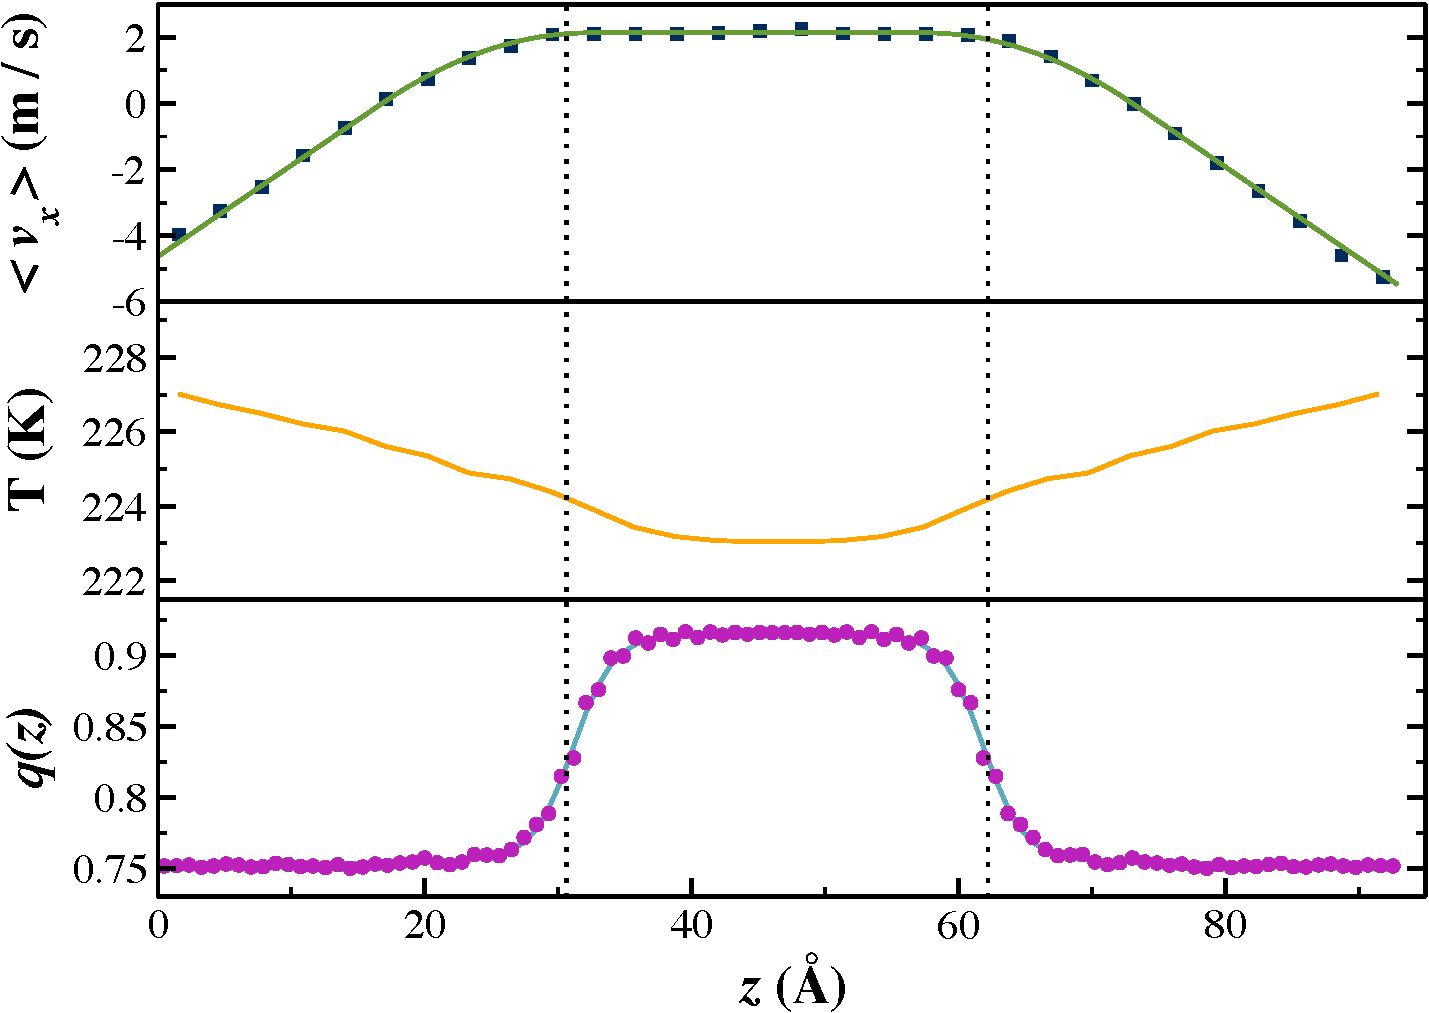
\includegraphics[width=\linewidth]{Figures/Pyr_comic_strip}
\caption{\label{fig:pyrComic} Properties of the SPC/E pyramidal
  interface being sheared through water at 7.6
  ms\textsuperscript{-1}. Lower panel: the local tetrahedral order
  parameter, $q(z)$, (circles) and the hyperbolic tangent fit
  (turquoise line).  Middle panel: the imposed thermal gradient
  required to maintain a fixed interfacial temperature of 225 K. Upper
  panel: the transverse velocity gradient (squares) that develops in
  response to an imposed momentum flux, along with the fit (green
  line). The vertical dotted lines indicate the locations of the Gibbs
  dividing surfaces of the two interfaces.}
\end{figure}

\begin{figure}
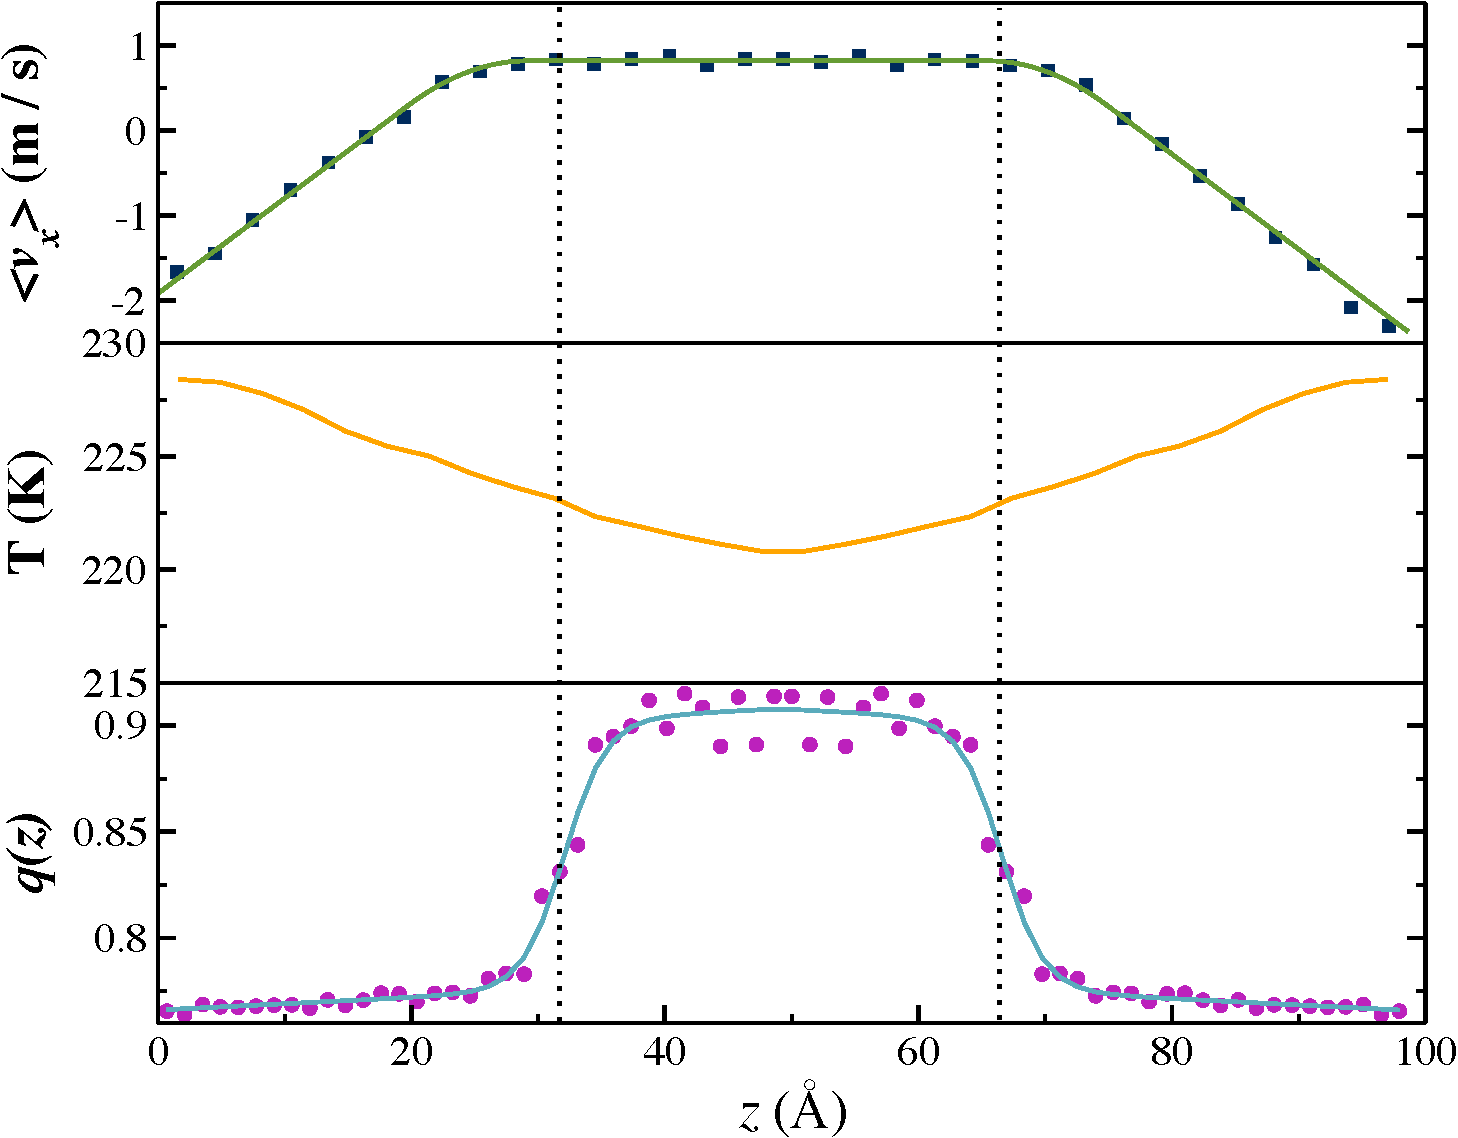
\includegraphics[width=\linewidth]{Figures/Bas_comic_strip}
\caption{\label{fig:bComic} Properties of the SPC/E basal interface being
  sheared through water at 3.2 ms\textsuperscript{-1}.  Panel
  descriptions are the same as in Fig. \ref{fig:pyrComic}.}
\end{figure}

\begin{figure}
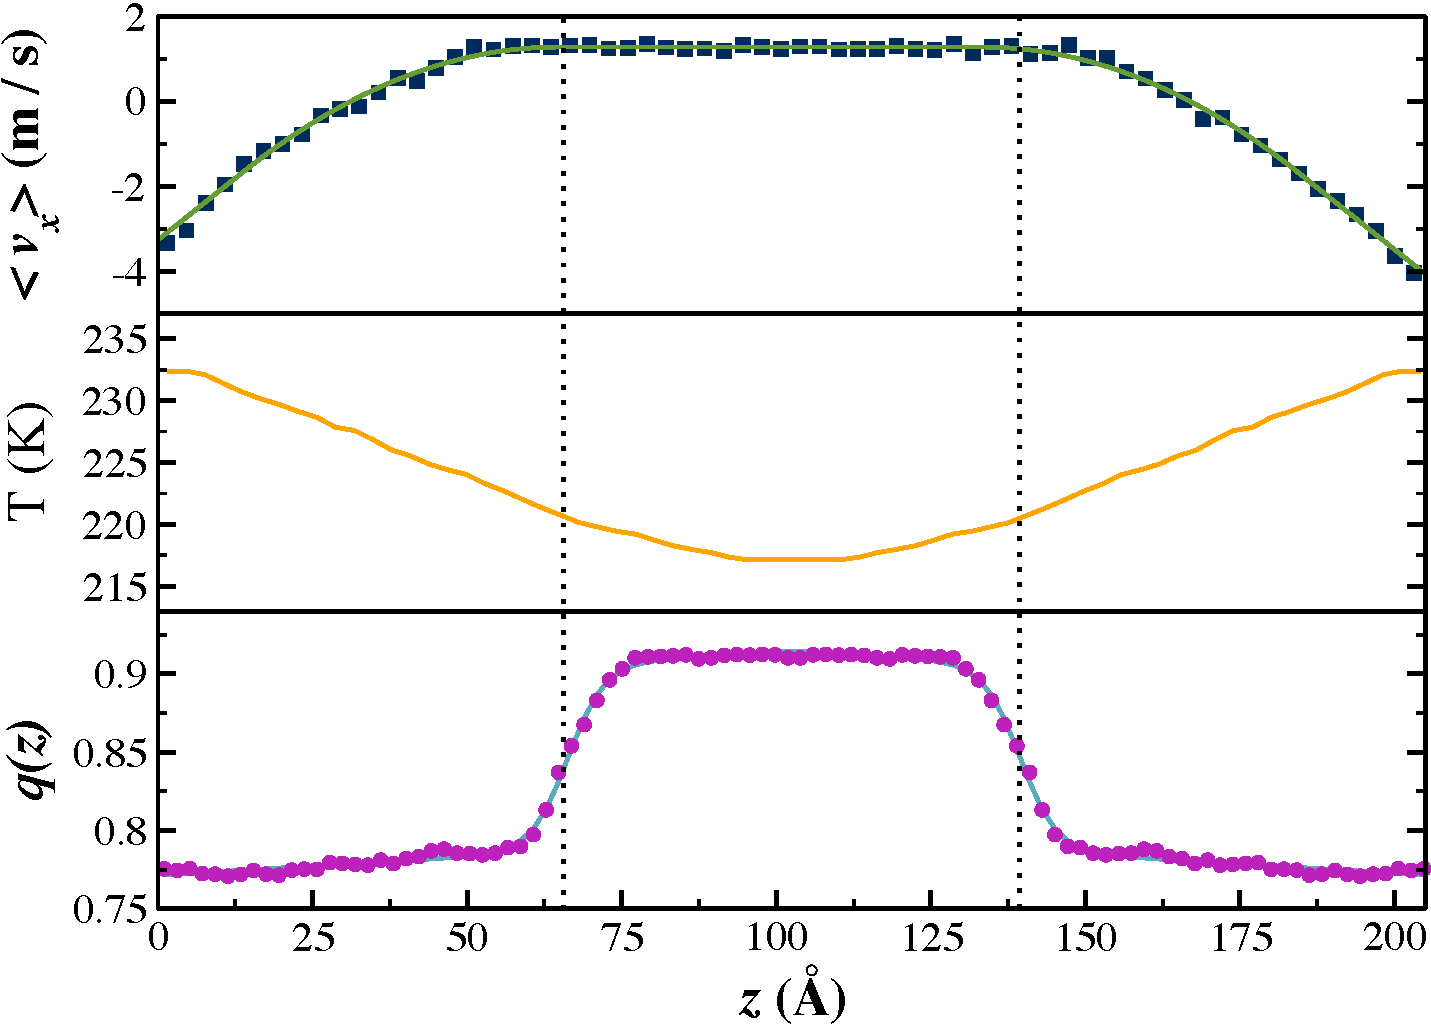
\includegraphics[width=\linewidth]{Figures/Pri_comic_strip}
\caption{\label{fig:pComic} Properties of the SPC/E prismatic interface
  being sheared through water at 6.0 ms\textsuperscript{-1}.  Panel
  descriptions are the same as in Fig. \ref{fig:pyrComic}.}
\end{figure}
%End figures of z-rnemd profile. 

%Begin rnemdz profiles for the TIP4P/Ice ice/water systems
\begin{figure}
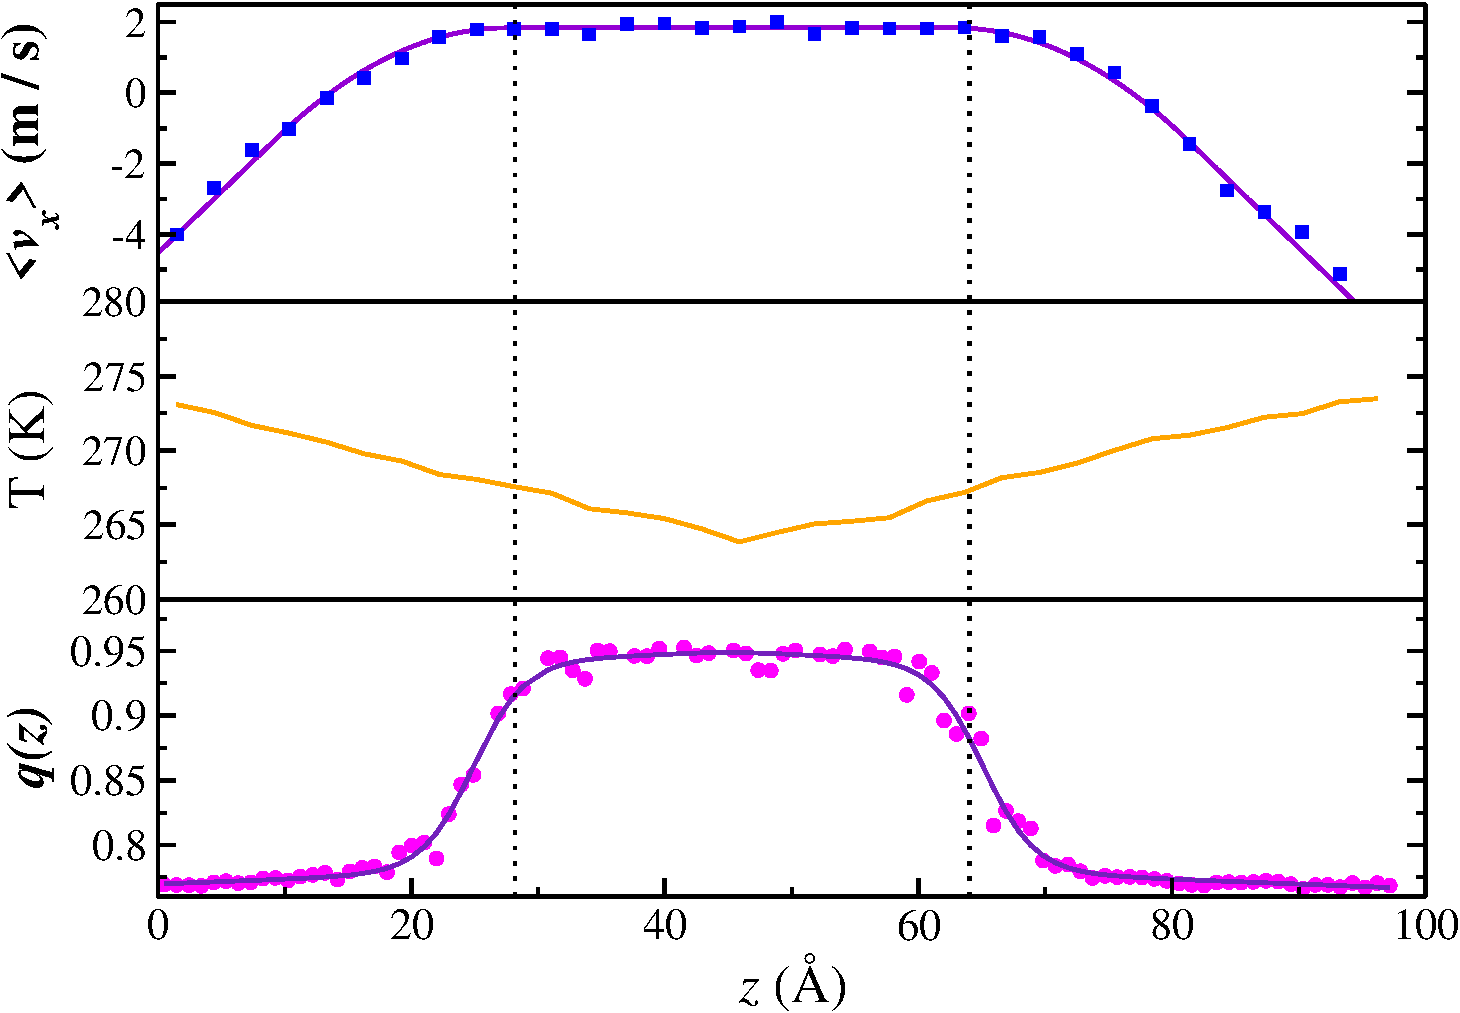
\includegraphics[width=\linewidth]{Figures/Basal_TIP4PIce_Plot}
\caption{\label{fig:tipbComic} Properties of the TIP4P/Ice Basal
  interface being sheared through water at 6.1
  ms\textsuperscript{-1}. Lower panel: the local tetrahedral order
  parameter, $q(z)$, (circles) and the hyperbolic tangent fit
  (blue line).  Middle panel: the imposed thermal gradient
  required to maintain a fixed interfacial temperature of 270 K. Upper
  panel: the transverse velocity gradient (squares) that develops in
  response to an imposed momentum flux, along with the fit (purple
  line). The vertical dotted lines indicate the locations of the Gibbs
  dividing surfaces of the two interfaces.}
\end{figure}

\begin{figure}
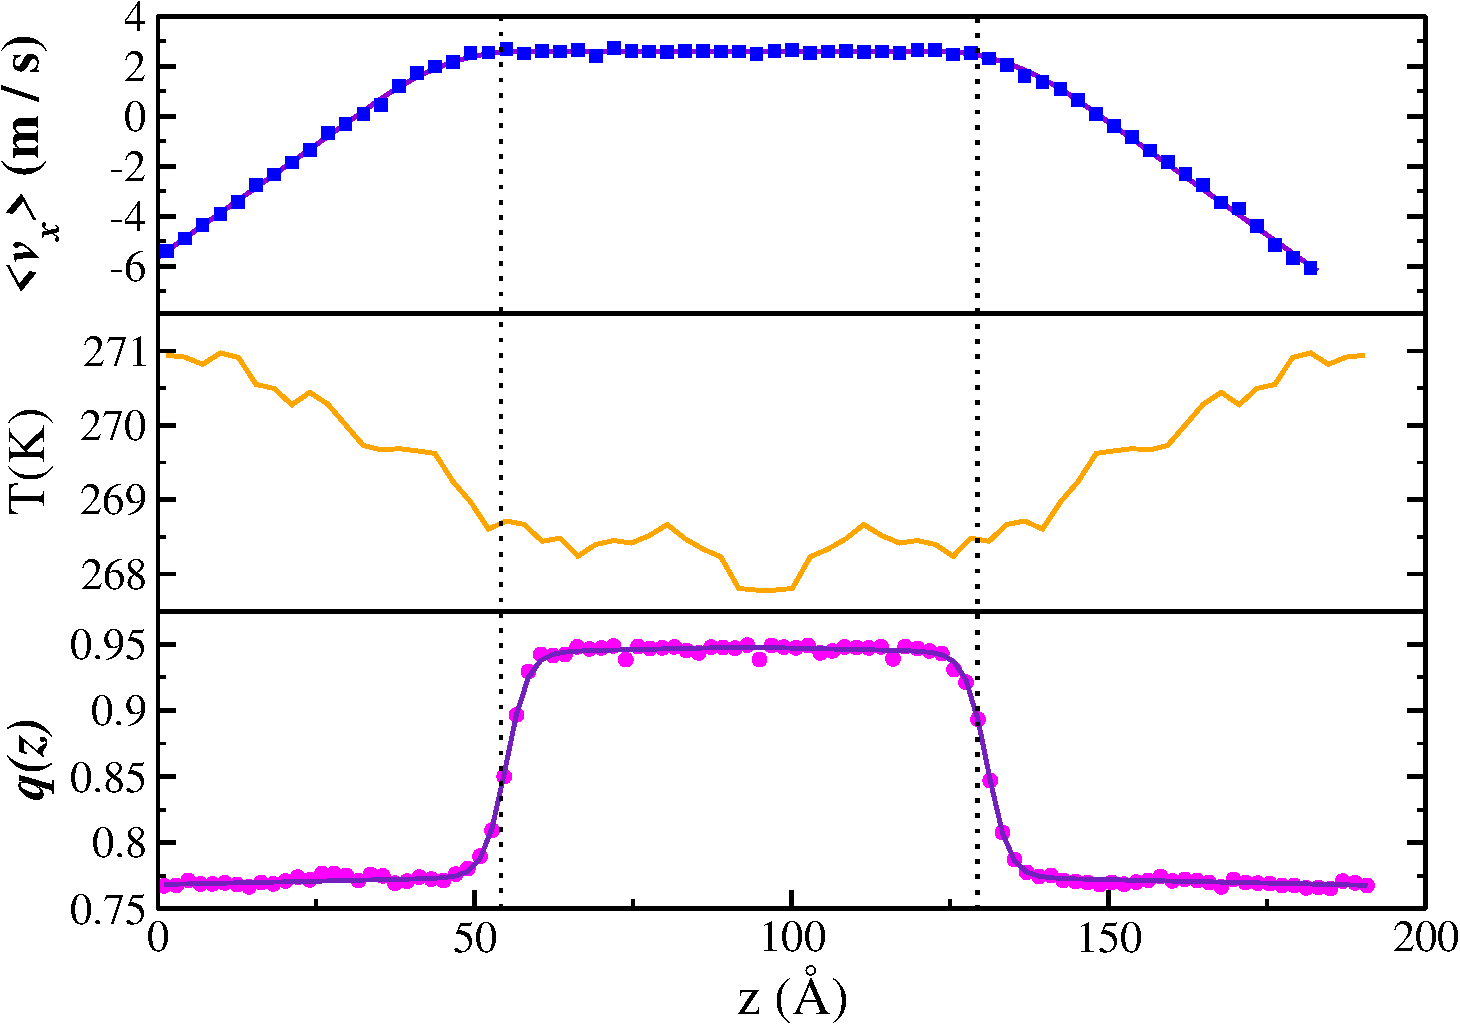
\includegraphics[width=\linewidth]{Figures/Prism_TIP4PIce_Plot}
\caption{\label{fig:tippComic} Properties of the TIP4P/Ice prismatic
  interface being sheared through water at 7.4 ms\textsuperscript{-1}.
  Panel descriptions are the same as in Fig. \ref{fig:tipbComic}.}
\end{figure}

\begin{figure}
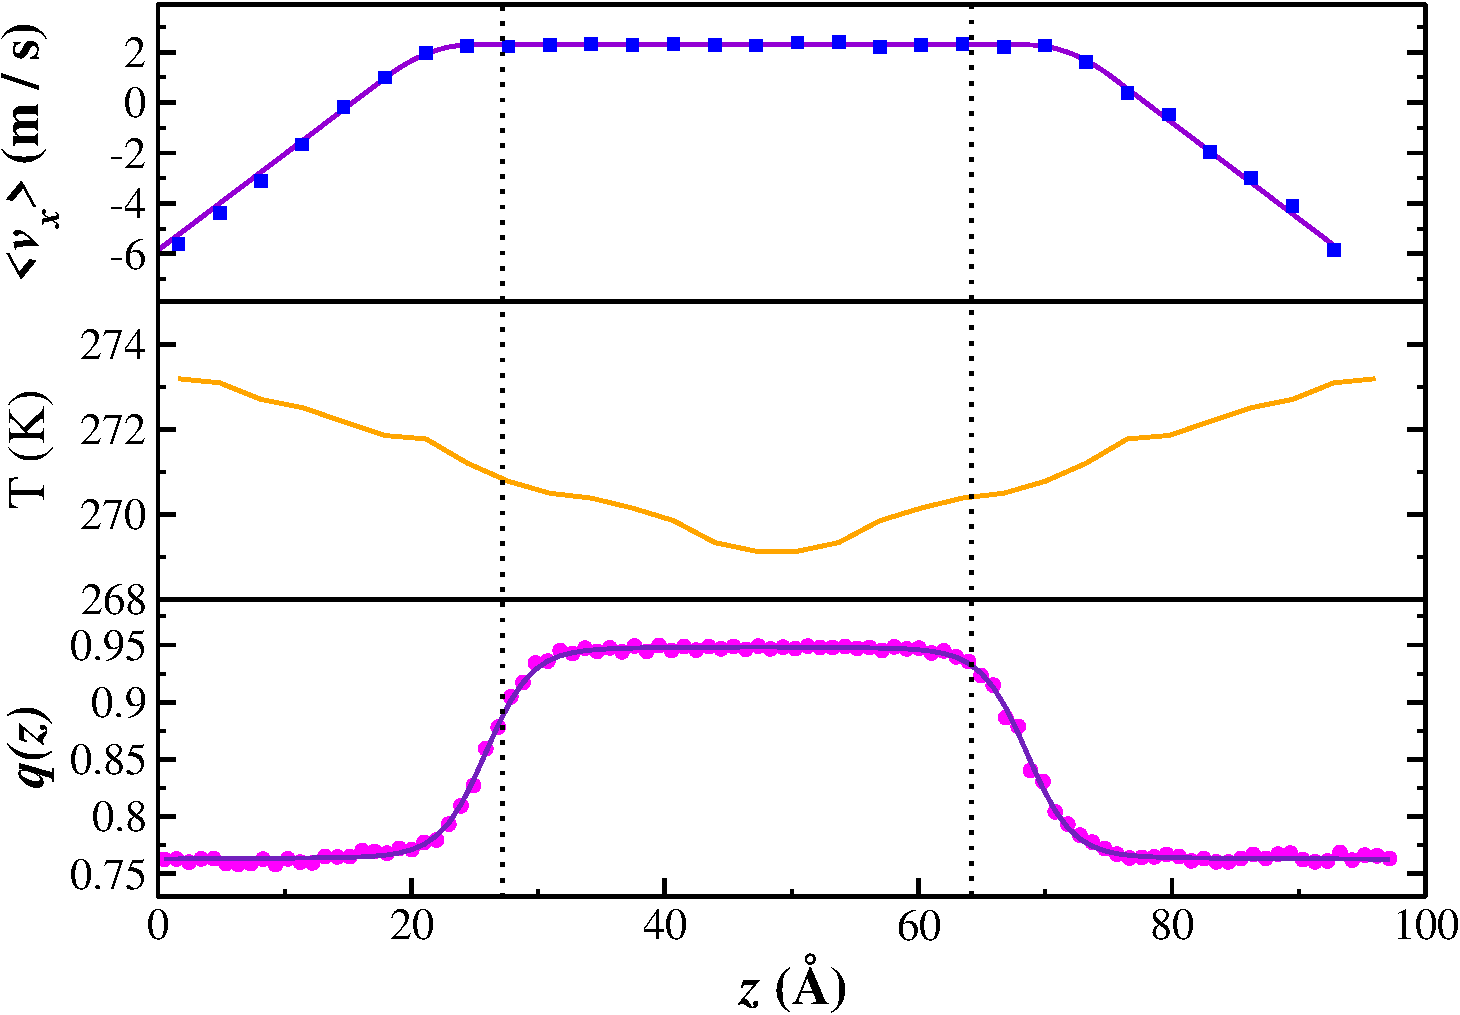
\includegraphics[width=\linewidth]{Figures/Pyra_TIP4PIce_Plot}
\caption{\label{fig:tippyComic} Properties of the TIP4P/Ice prismatic
  interface being sheared through water at 8.1 ms\textsuperscript{-1}.
  Panel descriptions are the same as in Fig. \ref{fig:tipbComic}.}
\end{figure}

\begin{figure}
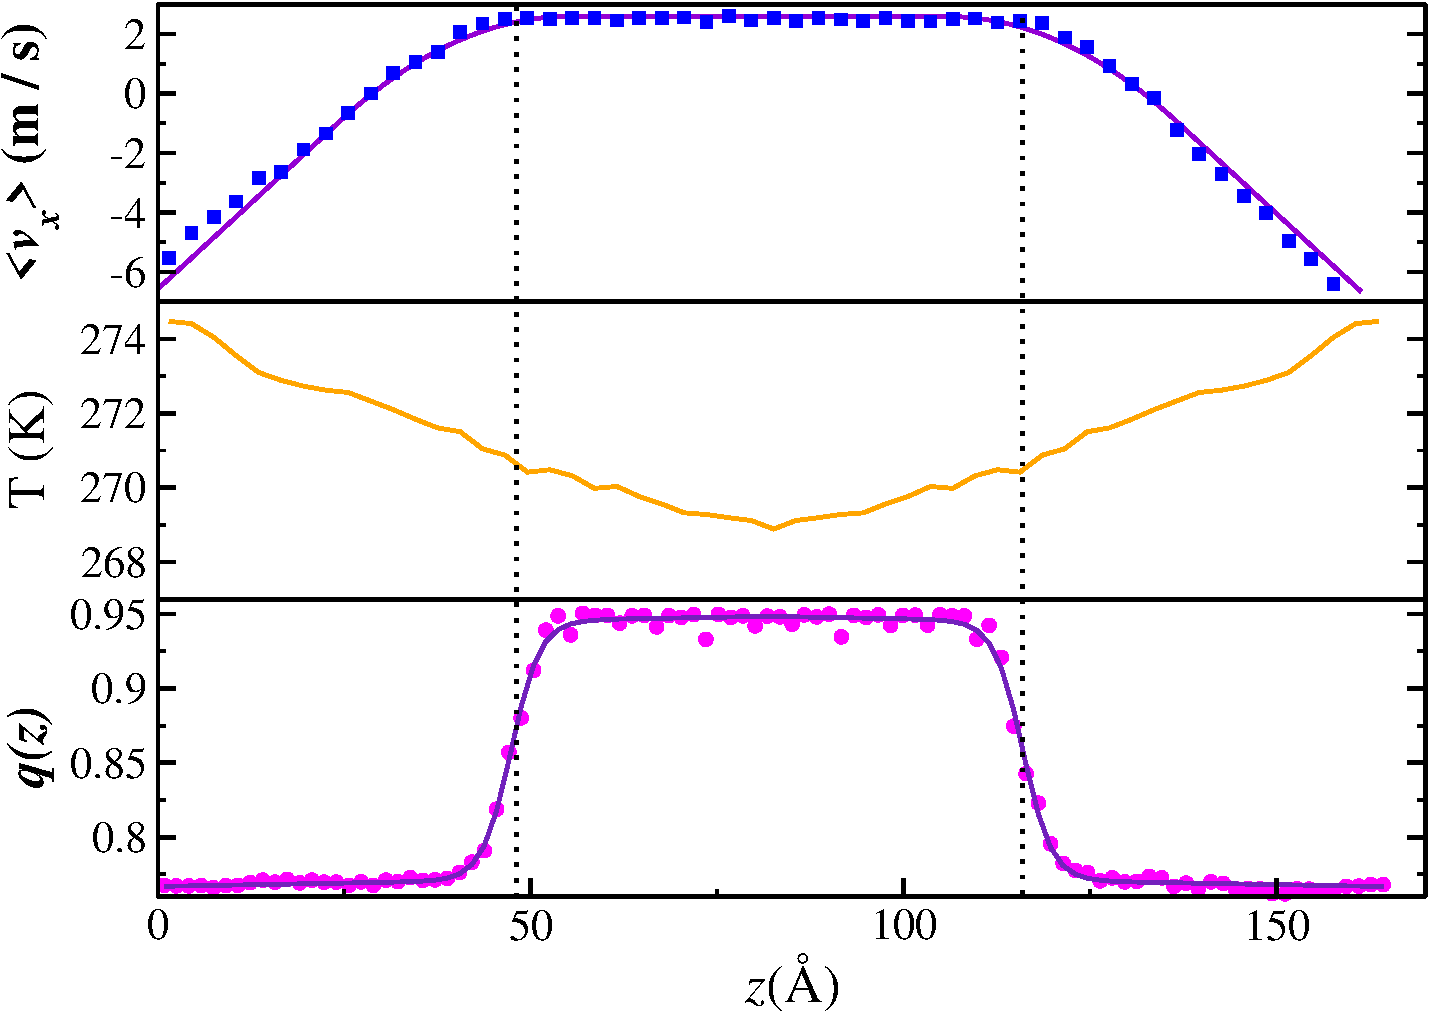
\includegraphics[width=\linewidth]{Figures/SecPrism_TIP4PIce_Plot}
\caption{\label{fig:tipsComic} Properties of the TIP4P/Ice secondary
  prism interface being sheared through water at 8.4
  ms\textsuperscript{-1}.  Panel descriptions are the same as in
  Fig. \ref{fig:tipbComic}.}
\end{figure}
%end TIP4P/Ice plots

%\section{Dependence of friction on Shear Rate}

\begin{figure}
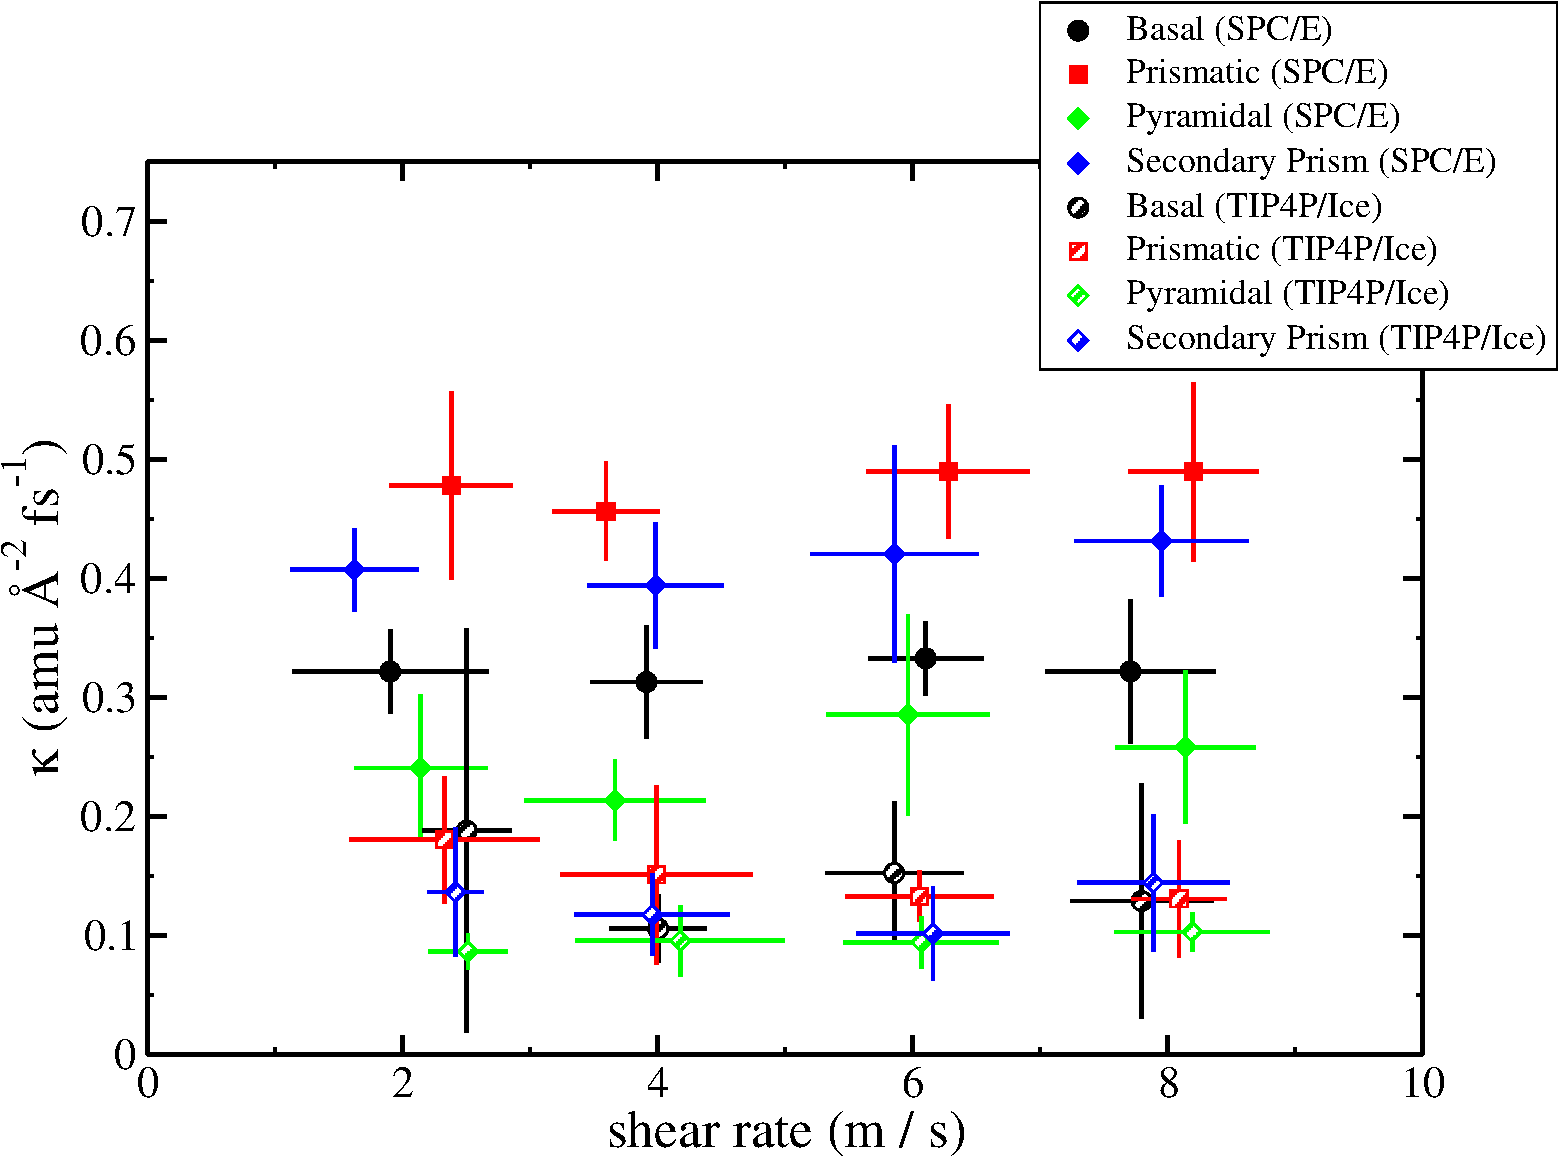
\includegraphics[width=\linewidth]{Figures/kappaPlot2}
\caption{\label{fig:kappaPlot} Dependence on the observed friction
  coefficient on the shear rate of the ice through the surrounding
  liquid water.  The RNEMD simulations impose a momentum flux, but the
  resulting shear rates can vary.  Here, we collect data in 2 m/s bins
  to accumulate statistics over multiple independent simulations.  The
  SPC/E simulations (solid symbols) were done at 225K, and the
  TIP4P/Ice simulations (patterned symbols) were carried out at
  270K. The points on this plot have also been averaged over shear
  direction ($x$ and $y$).}
\end{figure}


\newpage

\section{Projected Densities and Channel Widths}

In order to understand the behavior of liquid-phase water molecules
that are directly in contact with the four interfaces, we computed the
mean parallelepiped density,
\begin{equation}
\rho(y, z) = \frac{1}{L_x~dy~dz} \left< \sum_{i = 1}^{N} m_i \delta(y_i - y) \delta(z_i - z)\right>
\end{equation}
for four quiescent interfaces over 1 ns of simulation time (sampled
every ps).  Here, $dy$ and $dz$ are the lengths and widths of a set of
parallelepipeds that span the box depth ($L_x$), and for relatively
small $dy$ and $dz$ (0.05 \AA), the parallelepiped densities show the
smooth transition between the ordered ice facet and the surrounding
liquid.

\begin{figure}
\includegraphics[width=\linewidth]{Figures/DensityPlots}
\caption{\label{fig:DensPlots} Projected densities, $\rho(y, z)$, at
  the four quiescent interfaces.  Darker colors represent higher
  densities, while lighter colors (e.g. white) are relatively
  unpopulated.  For all four interfaces, the location of the
  tetrahedrality Gibbs dividing surface is indicated with a solid
  black line, while the two end points of the 90-10 width are shown in
  grey.}
\end{figure}

We note that the projected densities allow computation of the channel
widths and depth for the two prismatic facets using the locations of
the peak densities.  These figures also indicate that below the Gibbs
dividing surface, almost no liquid state molecules can be found
occupying the channels.

%Begin z-orientation times                                                      

\newpage   
\section{Orientational Decay Profiles}

\begin{figure}
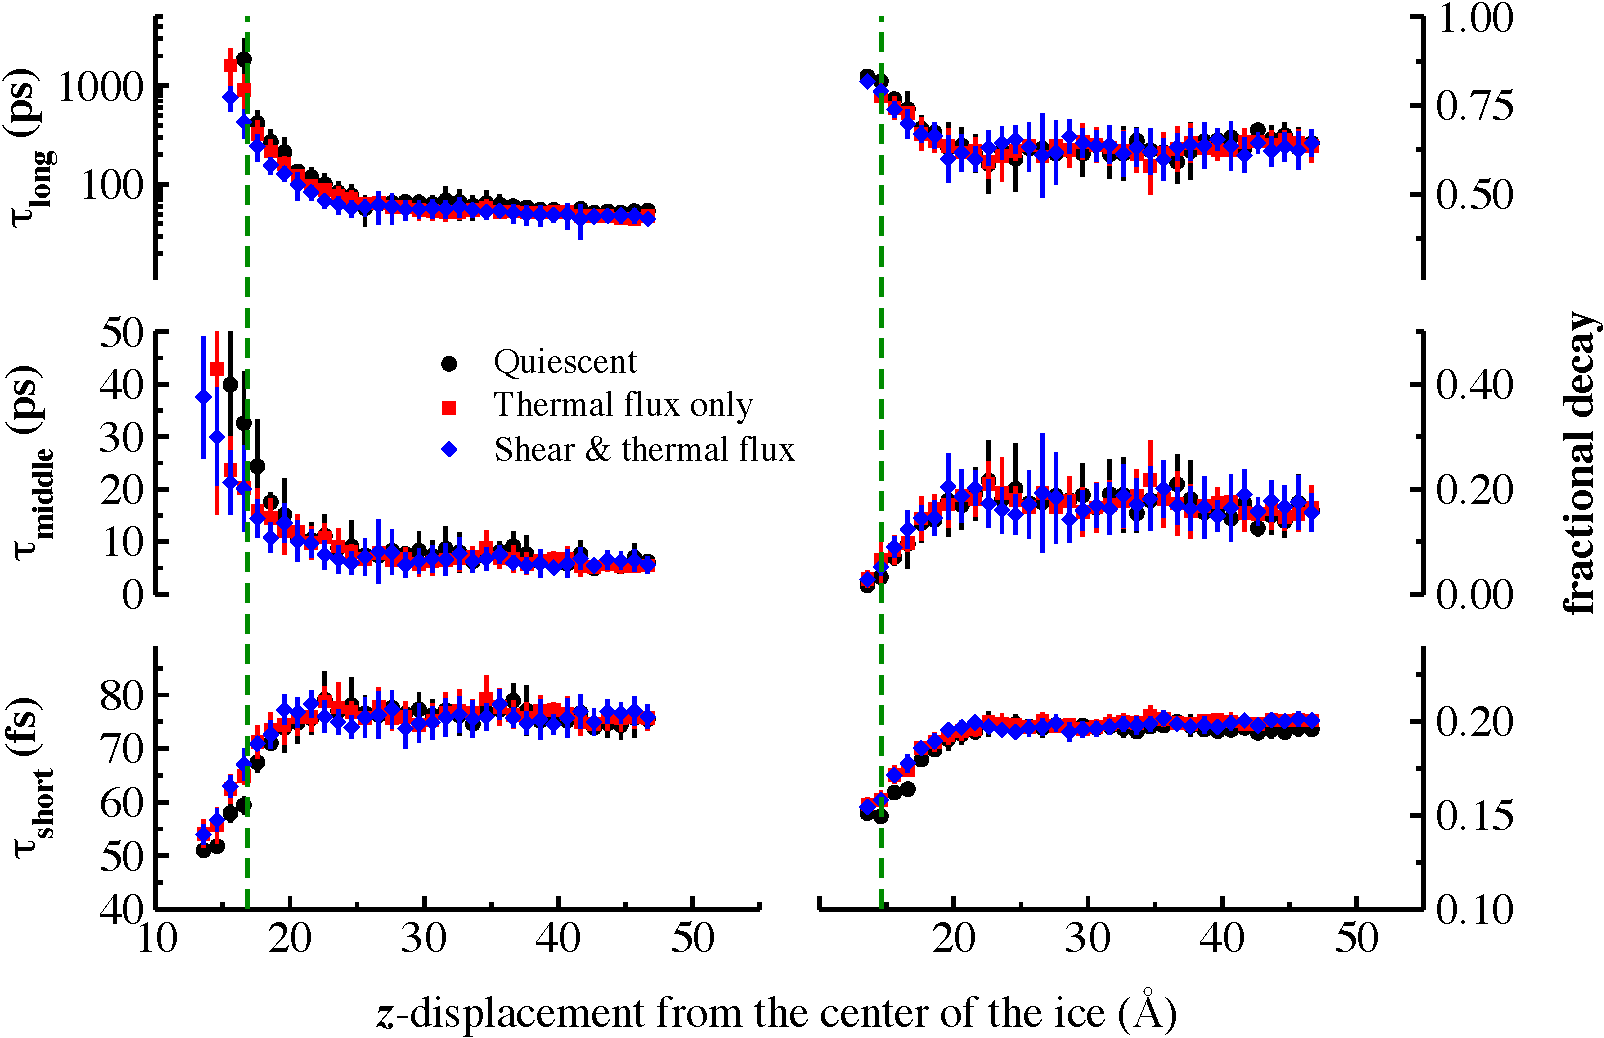
\includegraphics[width=\linewidth]{Figures/Pyr_lcorrz}
\caption{\label{fig:Pyrorient} Decay times (left) for $C_2(z,t)$ at
  the pyramidal interface, and their fractional contributions to the
  overall decay (right) fit using Eq. (8). The local decay constants
  are plotted as a function of distance from the center of the ice
  slab. The vertical dashed line indicates the Gibbs dividing surface
  determined using the local tetrahedral order parameter.  Results are
  shown for a quiescent system with no applied kinetic or momentum
  flux (black), an interface with with an imposed kinetic energy flux
  (red), and a sheared simulation (blue) with both kinetic and
  momentum fluxes.}
\end{figure}

\begin{figure}
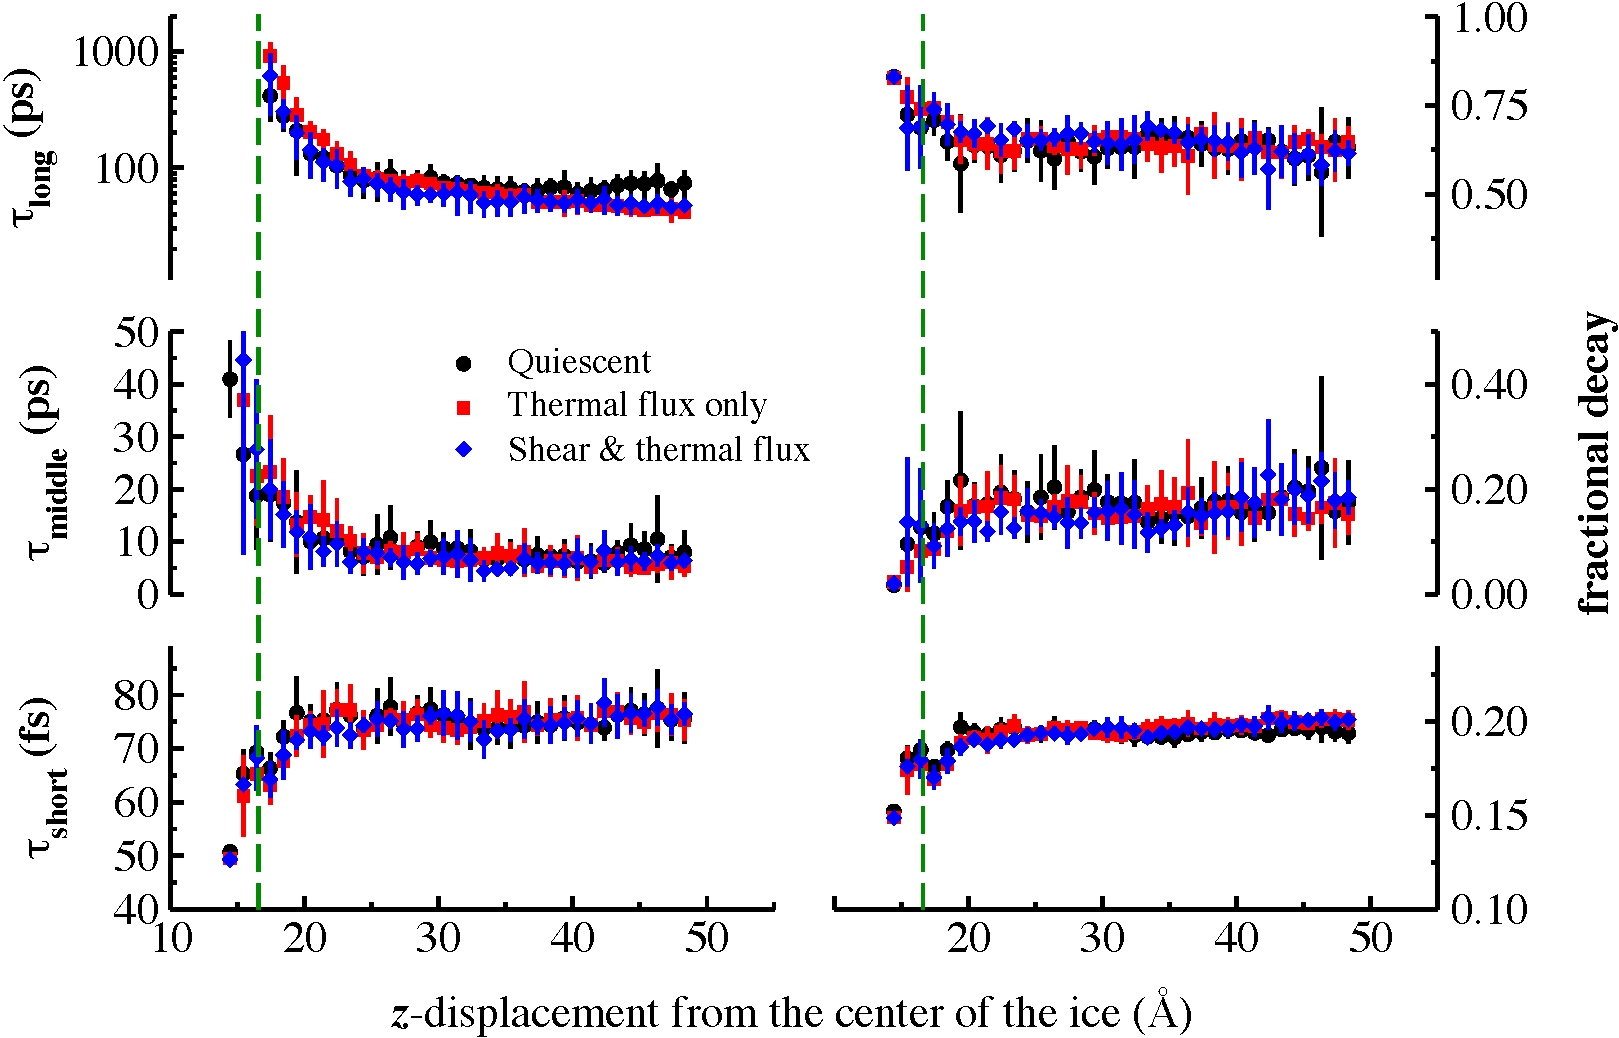
\includegraphics[width=\linewidth]{Figures/Bas_lcorrz}
\caption{\label{fig:Borient} $C_2(z,t)$ time constants for the basal
  interface.  Panel descriptions are the same as in
  Fig. \ref{fig:Pyrorient}. }
\end{figure}

\begin{figure}
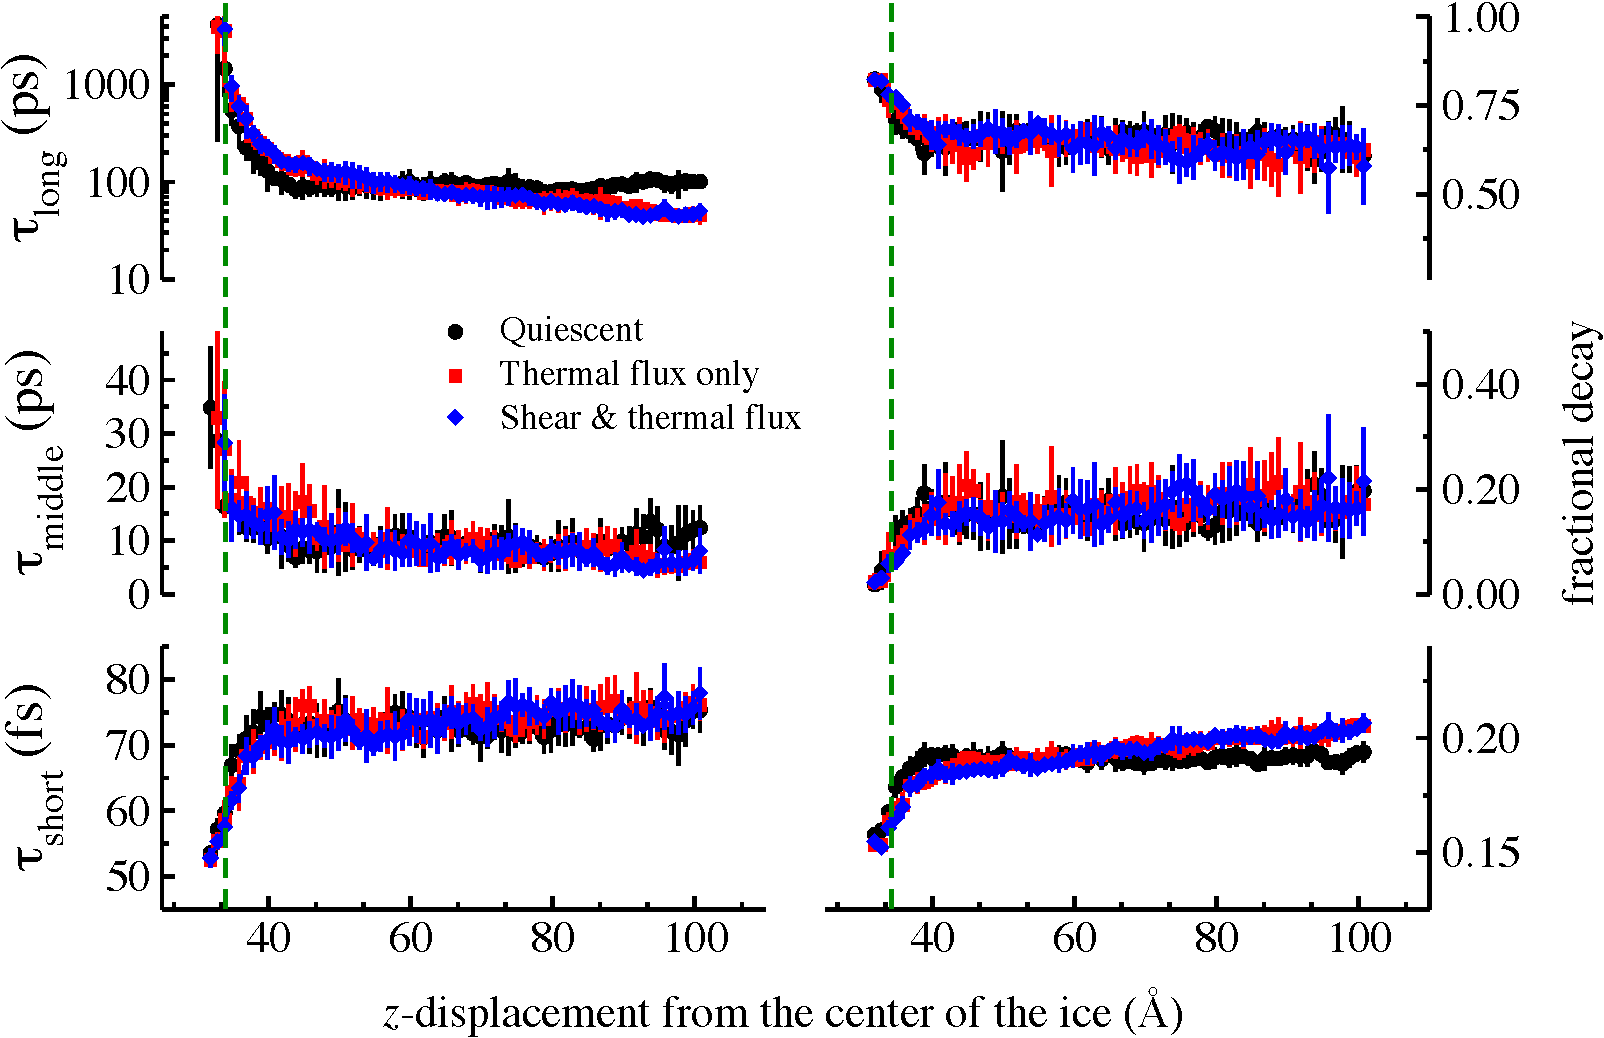
\includegraphics[width=\linewidth]{Figures/Pri_lcorrz}
\caption{\label{fig:Porient} $C_2(z,t)$ time constants for the prismatic
  interface.  Panel descriptions are the same as in
  Fig. \ref{fig:Pyrorient}.}
\end{figure}
%End z-orientation times       

\newpage
\section{Jump-time Decay Profiles}
\begin{figure}
\includegraphics[width=5.5in]{Figures/secPrismJumpPlot}
\caption{\label{fig:SPkjmp} Upper: Hydrogen bond jump correlation
  functions, $C_\mathrm{jump}(z,t)$, collected in 1 \AA~bins across
  the SPC/E secondary prism ice / water interface. The band that
  experiences very little decay represents water molecules in the ice,
  while the band that decays quickly corresponds to bins in the
  liquid.  The correlation function presents a continuous distribution
  of decay behaviors across the interface between ice and liquid
  water.  Lower: $C_\mathrm{jump}(z,t)$ decays exponentially, and each
  1 \AA~spatial bin can be fit with a jump rate, $k_\mathrm{jump}(z)$.
  These are shown with a fit that provides a ``jump'' width,
  $j_\mathrm{10-90}$. The locations of the structural Gibbs dividing
  surfaces (using tetrahedrality) are indicated with vertical dashed
  blue lines, while the locations of the ``jump'' interfaces are shown in
  orange.}
\end{figure}


\begin{figure}
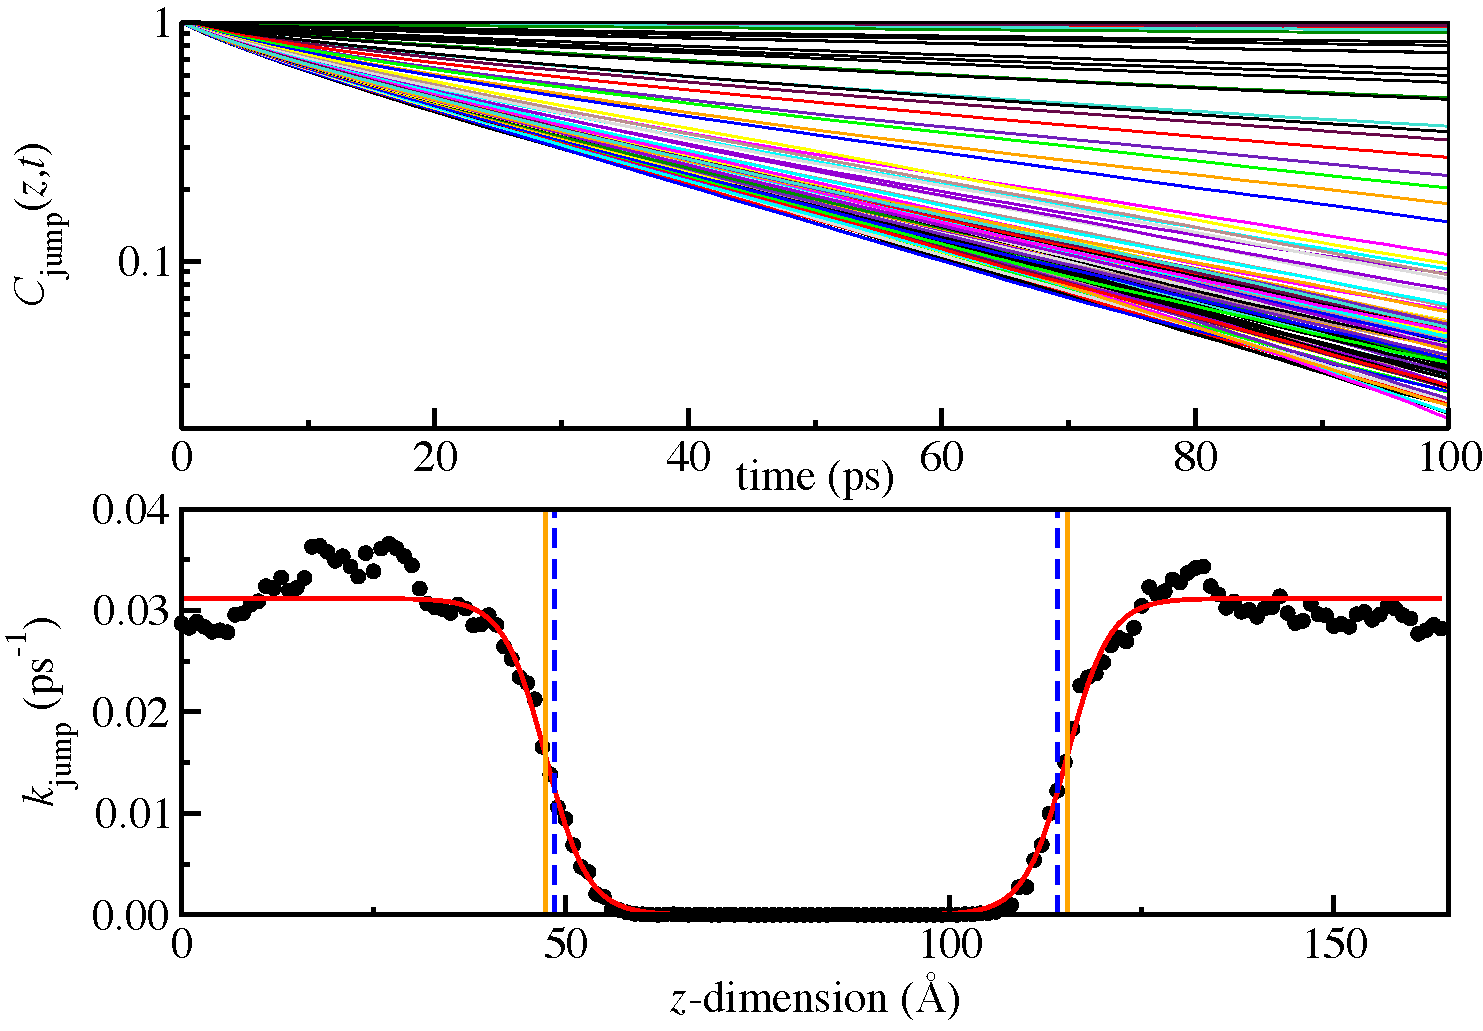
\includegraphics[width=\linewidth]{Figures/secprismJumpPlotTIP4PIce}
\caption{\label{fig:SPTIP4Pkjmp} The same secondary prism hydrogen
  bond jump data as Fig. \ref{fig:SPkjmp}, but collected using the
  TIP4P/Ice model and at 270~K.  Note that the higher coexistence
  temperature for this model increases the observed liquid-state jump
  rates, and has brought the structural and jump interfaces much
  closer together.}
\end{figure}
